% \documentclass[oneside]{report}
\documentclass[oneside,final,14pt,a4paper]{extreport}
% \documentclass[journal,onecolumn,a4paper,12pt]{IEEEtran}
\usepackage[T2A]{fontenc}


\usepackage{vmargin}
\setpapersize{A4}
\setmarginsrb{2.5cm}{2cm}{2cm}{2cm}{0pt}{10mm}{0pt}{13mm}
\usepackage{setspace}
\sloppy
\setstretch{1.5}
\usepackage{indentfirst}
\parindent=1.25cm

%%%%% ADDED TO SUPPORT TT BOLD FACES %%%%
\DeclareFontShape{OT1}{cmtt}{bx}{n}{<5><6><7><8><9><10><10.95><12><14.4><17.28><20.74><24.88>cmttb10}{}
\renewcommand{\ttdefault}{pcr}
%%%%% END %%%%%%%%%%%%%%%%%%%%%%%%%%%%%%% 
\usepackage{atbegshi,picture}
\AtBeginShipout{\AtBeginShipoutUpperLeft{%
  \put(\dimexpr\paperwidth-1cm\relax,-1.5cm){\makebox[0pt][r]{
\includegraphics[width=3cm]{figs/inno}}}%
}}


\usepackage[english]{babel}
\usepackage[backend=biber,style=ieee,autocite=inline]{biblatex}
\bibliography{ref.bib}
\DefineBibliographyStrings{english}{%
  bibliography = {References},}
\usepackage{blindtext}
\usepackage{pdfpages}
\newenvironment{bottompar}{\par\vspace*{\fill}}{\clearpage}
\usepackage{amsmath,amsfonts}
\usepackage{url}

\usepackage{amsthm}
\newtheorem{theorem}{Theorem}
\newtheorem{corollary}{Corollary}
\newtheorem{lemma}{Lemma}
\newtheorem{proposition}{Proposition}
\theoremstyle{definition}
\newtheorem{definition}{Definition}
\theoremstyle{remark}
\newtheorem*{remark}{Remark}
\theoremstyle{remark}
\newtheorem*{example}{Example}


\usepackage{titlesec}
\usepackage{float}
\usepackage{graphicx}
\graphicspath{{figs/}} %path to images
\usepackage{array}
\usepackage{multirow,array}
\usepackage{caption}
\usepackage{subcaption}
\usepackage{hyperref}
\usepackage{paralist}
\usepackage{listings}
\usepackage{zed-csp}
\usepackage{fancyhdr}
\usepackage{csquotes}
\usepackage{color}
\usepackage{anyfontsize}
\usepackage{mathptmx}
\usepackage{t1enc}
\usepackage{syntax}
\usepackage{chngcntr}
\usepackage{upgreek} 
\usepackage{bm}
% \usepackage{hyperref}
\usepackage{multicol}
\usepackage{setspace}
\usepackage{booktabs}
\usepackage{multirow}
\usepackage{longtable}
\usepackage[font=singlespacing, labelfont=bf]{caption}
\counterwithout{table}{chapter}
\renewcommand{\thetable}{\Roman{table}}
%Hints
\newcommand\pic[1]{(Fig. \ref{#1})} %Ref on figure
\newcommand\tab[1]{(Tab. \ref{#1})} %Ref on table

\setlength{\headheight}{32.0976pt}
\usepackage{enumitem}
\newlist{inlinelist}{enumerate*}{1}
\setlist*[inlinelist,1]{%
  label=(\arabic*),
}

\usepackage{cleveref}
\crefname{table}{table}{tables}
\Crefname{table}{Table}{Tables}
\crefname{figure}{Fig.}{figures}
\Crefname{figure}{Fig.}{Figures}
\crefname{listing}{List.}{List.}
\Crefname{listing}{List.}{List.}

% --- START --- minted

% https://github.com/latextemplates/IEEE/blob/main/paper-conference-minted.tex
\usepackage[newfloat]{minted}
\setminted{
  % Add line numbers, can be added per listing 
  % linenos=true,
  % Line numbers not flowing out of the margin
  numbersep=12pt,
  xleftmargin=19pt,
  breaklines=true,
  breakbytoken=true,
  % For the very long tokens, use
  % "breakanywhere, breakbytokenanywhere=false"
  % on the listing level. Otherwise breakanywhere will not have any effect.
  breakbytokenanywhere=true
}
\renewcommand{\theFancyVerbLine}{\textcolor{gray}{\arabic{FancyVerbLine}}}

\captionsetup[listing]{labelfont={normalfont}, name={List.}, labelsep=period}
\counterwithout{listing}{chapter}

\newcommand{\hs}{\mintinline[fontsize=\normalsize]{haskell}}

\newcommand{\clerk}{\texttt{clerk} }

% --- END --- minted

\setcounter{secnumdepth}{4}
\captionsetup[table]{labelfont={normalfont}, name={TABLE}, labelsep={newline}}
\counterwithout{table}{chapter}
\renewcommand{\thetable}{\Roman{table}}
\setlength{\parindent}{2em} 
\DeclareCaptionLabelSeparator{figSep}{.\quad}
\captionsetup[figure]{labelfont={normalfont}, name={Fig.}, labelsep=period}
\counterwithout{figure}{chapter}

\titleformat{\section}[hang]{\fontsize{20}{24}\selectfont\filcenter}{\Roman{section}}{1em}{}
\titleformat{\subsection}[hang]{\itshape}{\Alph{subsection}.}{1em}{}[]
\titleformat{\subsubsection}[runin]{\itshape}{\arabic{subsubsection})}{1em}{}[$:$]
\titlespacing{\subsubsection}{1em}{1em}{1em}
\titleformat{\paragraph}[runin]{\itshape}{\alph{paragraph})}{1em}{}[$:$\quad]
\titlespacing{\paragraph}{2em}{1em}{1em}

\pagestyle{fancyplain}

% remember section title
\renewcommand{\chaptermark}[1]%
	{\markboth{\chaptername~\thechapter~--~#1}{}}

% subsection number and title
\renewcommand{\sectionmark}[1]%
	{\markright{\thesection\ #1}}

\rhead[\fancyplain{}{\bf\leftmark}]%
      {\fancyplain{}{\bf\thepage}}
\lhead[\fancyplain{}{\bf\thepage}]%
      {\fancyplain{}{\bf\rightmark}}
\cfoot{} %bfseries


\newcommand{\dedication}[1]
   {\thispagestyle{empty}
     
   \begin{flushleft}\raggedleft #1\end{flushleft}
}

\begin{document}

%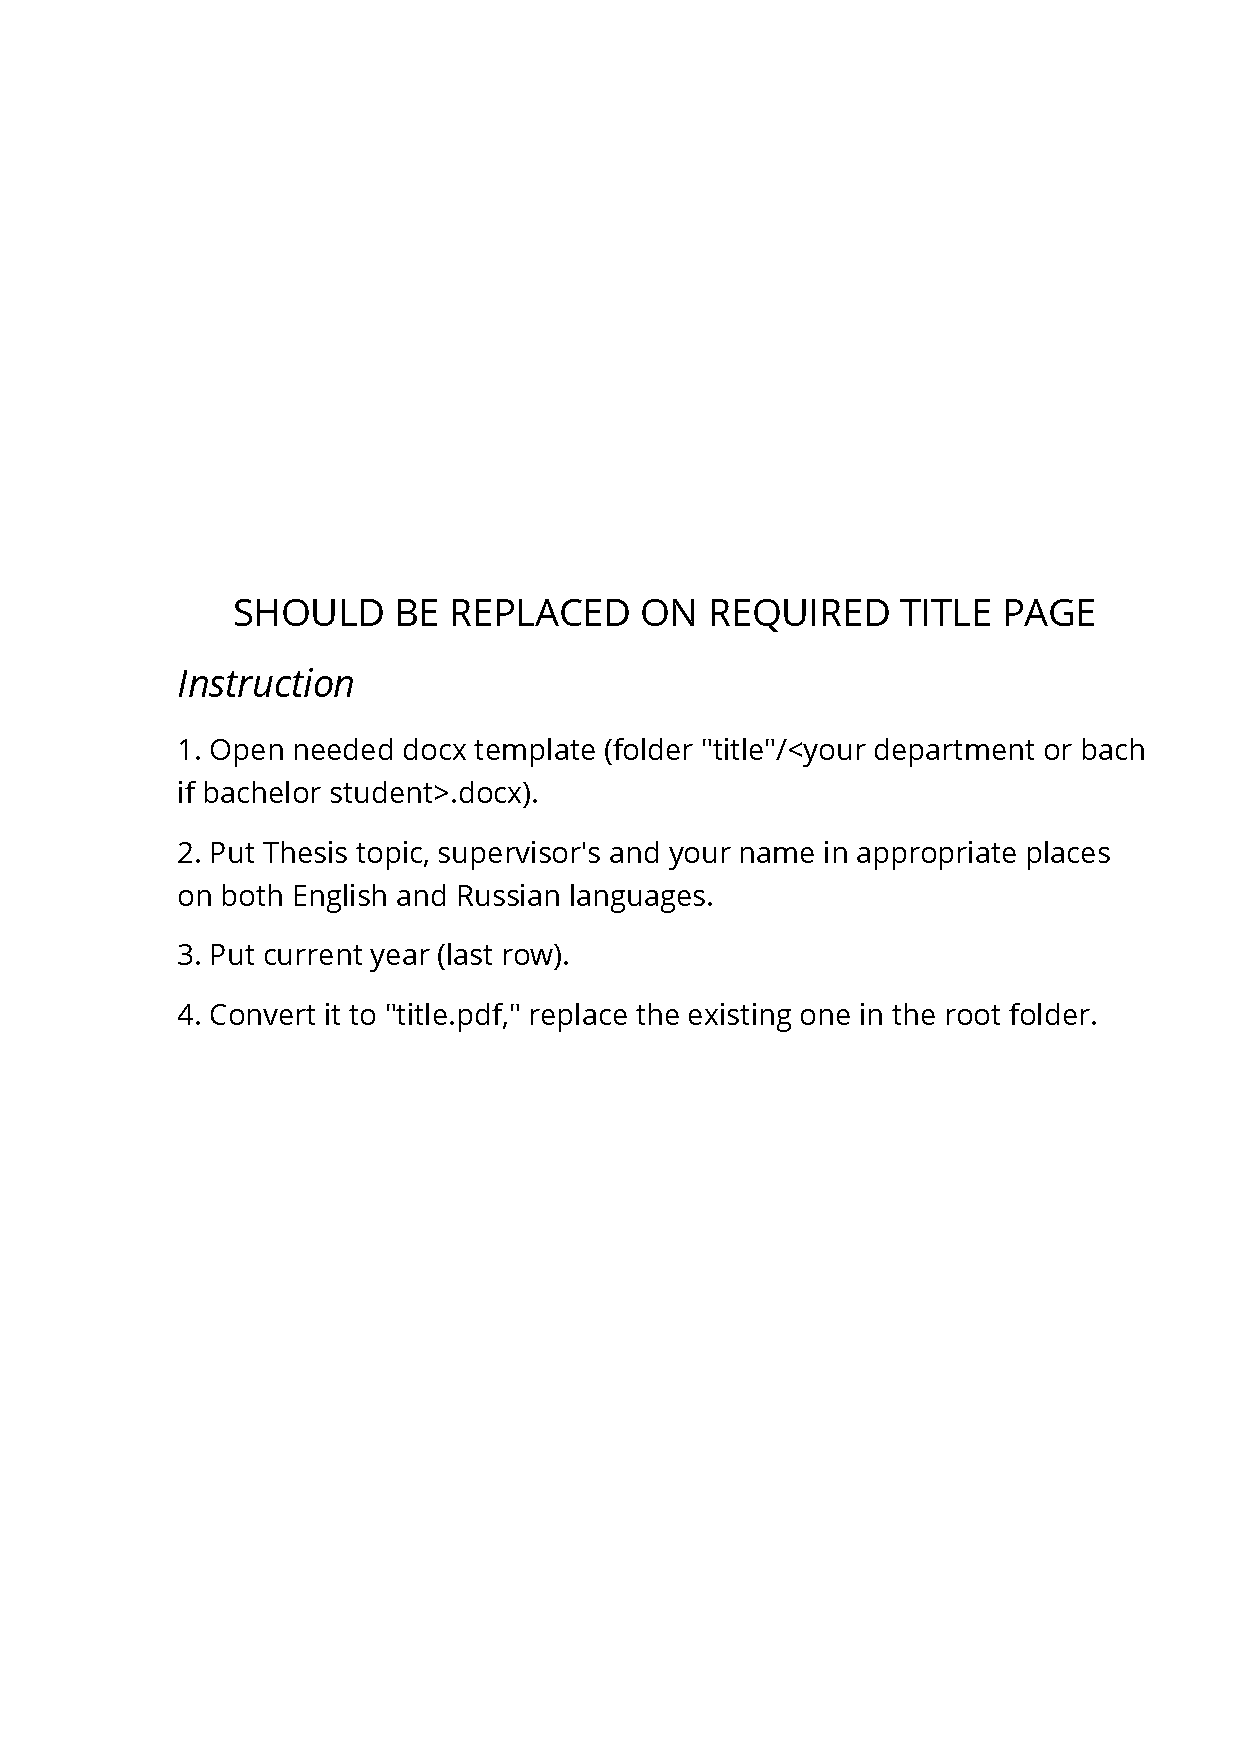
\includepdf[pages=-]{title.pdf}
%\tableofcontents
%\listoftables
%\listoffigures


\newpage
%\begin{abstract}
abstract \ldots
\end{abstract}
% Depend on above part
\setcounter{page}{1}
% \chapter{Введение}
\label{chap:intro}

%\chapter{Literature Review}
\label{chap:lr}
\chaptermark{Second Chapter Heading}


\Blindtext[2]

\section{Another Section}
\Blindtext[1]
\newpage
With the widespread of computing systems, information processing, and net working, the practice of replacing paper documentation to electronic documentation has become more and more common. Electronic documentation within the workplace has several advantages over the traditional one, such as being easy to share, copy and edit the document. However, these advantages also present a problem. A malefactor, having access to the system, can easily copy and leak the document, without leaving any trace. Such actions are virtually undetectable in most systems, so, the malefactor goes unpunished. In this thesis, we propose one solution to the problem: digital watermarking. 

Every electronic document within the protected system is marked with an invisible digital watermark, containing information about the user, accessing this particular document. Therefore, in case the protected company discovers the leaked document, they will be able to identify the machine of the malicious person and time when the document was leaked. This will allow inflicting punishment on the malefactor, recovering the costs of the leak, and potentially preventing future ones. 

\begin{longtable}{c|c}
\caption[This is the title I want to appear in the List of Tables]{Simulation Parameters} \label{table:secsimulation_params} \\
\hline
A & B  \\
\hline
\endfirsthead
\multicolumn{2}{@{}l}{} \\
\hline
A & B \\
\hline
\endhead
\hline
 \textbf{Parameter} & \textbf{Value}\\
 \hline
 Number of vehicles & $|\mathcal{V}|$\\
 \hline
 Number of RSUs & $|\mathcal{U}|$\\
 \hline
 RSU coverage radius & 150 m\\
 \hline
 V2V communication radius & 30 m\\
 \hline
 Smart vehicle antenna height & 1.5 m\\
 \hline
 RSU antenna height & 25 m\\
 \hline
 Smart vehicle maximum speed & $v_{max}$ m/s\\
 \hline
 Smart vehicle minimum speed & $v_{min}$ m/s\\
 \hline
 Common smart vehicle cache capacities & $[50, 100, 150, 200, 250]$ mb\\
 \hline
 Common RSU cache capacities & $[5000,1000,1500,2000,2500]$ mb\\
 \hline
 Common backhaul rates & $[75, 100, 150]$ mb/s\\
 \hline
\end{longtable}

\begin{figure}[hbt]
\centering

\includegraphics[]{figs/inno.png}
\caption{One kernel at $x_s$ (\emph{dotted kernel}) or two kernels at
$x_i$ and $x_j$ (\textit{left and right}) lead to the same summed estimate
at $x_s$. This shows a figure consisting of different types of
lines. Elements of the figure described in the caption should be set in
italics, in parentheses, as shown in this sample caption.}
\label{fig:secex}
\end{figure}

This description implies several essential properties of the task at hand:
\begin{enumerate}
    \item Watermark must contain all necessary information, but still, be placeable and recognizable even on smaller images. The produced watermark must be compact but have the possibility to store enough information. 
    \item To prevent easy tampering, the watermark must be invisible to the naked eye (and, preferably, to basic image parsing tools). If malefactor does not know about the existence of watermark, they might not even try to remove it and disable it. 
\end{enumerate}

% % LIMA_DISABLE

% {- FOURMOLU_DISABLE -}
% {-# OPTIONS_GHC -Wno-redundant-constraints #-}
% {-# LANGUAGE OverloadedStrings #-}
% {-# LANGUAGE DerivingVia #-}
% {-# LANGUAGE ScopedTypeVariables #-}
% {-# LANGUAGE ViewPatterns #-}
% {-# LANGUAGE RecordWildCards #-}
% {-# LANGUAGE UndecidableInstances #-}
% {-# LANGUAGE DeriveAnyClass #-}
% {-# LANGUAGE MonoLocalBinds #-}
% {- FOURMOLU_ENABLE -}

% -- | @Clerk@ library
% module Clerk (
%   -- * Coords
%   Coords,
%   mkCoords,
%   ToCoords (..),
%   FromCoords (..),
%   IsCoords,

%   -- * Cell references
%   Ref,
%   row,
%   col,
%   ref,
%   val,

%   -- * Changing types
%   UnsafeChangeType (..),
%   as,

%   -- * Cell formatting
%   InputIndex,
%   FormatCell,
%   CellTemplate,
%   FormattedMap,
%   FMTransform,
%   WSTransform,
%   Transform,
%   FCTransform,
%   horizontalAlignment,
%   mkColor,
%   blank,
%   ToARGB (..),

%   -- * Templates
%   Row,
%   RowI,
%   RowIO,
%   Template,

%   -- * Columns
%   ColumnsProperties,
%   columnWidthFormatRef,
%   columnWidthRef,
%   columnWidth,
%   columnRef,
%   column,

%   -- * Sheet builder
%   Sheet,
%   placeN,
%   place1,
%   place,
%   evalSheetDefault,

%   -- * Expressions
%   Expr,
%   Formula,
%   ToFormula (..),
%   NumOperator,
%   (.+),
%   (.-),
%   (.*),
%   (./),
%   (.:),
%   (.^),
%   (.^^),
%   (.**),
%   (.<),
%   (.>),
%   (.<=),
%   (.>=),
%   (.=),
%   (.<>),
%   (.&),
%   fun,
%   -- TODO work on default types
%   Range,
%   FunName,

%   -- * Cells
%   CellData,
%   ToCellData (..),

%   -- * xlsx
%   composeXlsx,
%   writeXlsx,

%   -- * For examples
%   SheetState (..),
%   RowState,
%   RowShow (..),
%   evalRow,
%   mkRef,
%   showFormula,
% ) where

% import Codec.Xlsx qualified as X
% import Codec.Xlsx.Formatted qualified as X
% import Control.Monad (forM, void, zipWithM)
% import Control.Monad.State (MonadState, StateT (StateT), evalStateT, get, gets, modify)
% import Control.Monad.Trans.Writer (execWriter, runWriter)
% import Control.Monad.Writer (MonadWriter (..), Writer)
% import Data.ByteString.Lazy qualified as LBS
% import Data.Char (isAlpha, ord)
% import Data.Default (Default (..))
% import Data.Foldable (Foldable (..))
% import Data.Kind (Type)
% import Data.Map.Strict qualified as Map (Map, insert)
% import Data.Maybe (isJust, maybeToList)
% import Data.Text (Text)
% import Data.Text qualified as T
% import Data.Time.Clock.POSIX (getPOSIXTime)
% import GHC.Generics (Generic)
% import Lens.Micro (Lens', lens, (%~), (&), (+~), (.~), (?~), (^.))
% import Unsafe.Coerce (unsafeCoerce)

% LIMA_ENABLE

This chapter describes low-level details of the \texttt{clerk} library implementation. First, the used types and their purpose are explained. Following that, the main helper functions are presented. Finally, a simple example is given to demonstrate the capabilities of \texttt{clerk}.

\section{Imports}

Here are the necessary imports.

% SINGLE_LINE FOURMOLU_DISABLE

% SINGLE_LINE FOURMOLU_ENABLE

\section{Types}
\label{sec:types}

The core type of the library is \texttt{Row}. This is a monad for construction of a template for a row of data. It keeps track of the coordinates of the current cell via the \texttt{StateT Coords m a} transformer. It writes the new cells into a template via the \texttt{Writer (Template input output) a}.

\begin{mycode}
newtype RowIO input output a = Row
  {unRow :: StateT RowState (Writer (Template input output)) a}
  deriving newtype (Functor, Applicative, Monad, MonadState RowState, MonadWriter (Template input output))

type RowState = Coords
\end{mycode}

The row templates are applied to a list of inputs, producing a template for a table.
In this table, each cell has an address, data, and formatting. A special type is used to construct formulas to produce data.

\subsection{Addresses}
\label{sec:addresses}

The \texttt{Coords} denote the address of a cell. This data type has a \texttt{Num} instance that provides cell arithmetics with them like shifts along sheet axes in the directions given as another \texttt{Coords}. Additionally, this type has a \texttt{Show} instance that translates it into valid spreadsheet addresses.

\begin{mycode}
data Coords = Coords
  { _col :: Int
  , _row :: Int
  , _coordsWorksheetName :: T.Text
  , _coordsWorkbookPath :: FilePath
  }
  deriving (Generic, Default, Show)
\end{mycode}

Typeclasses \texttt{ToCoords} and \texttt{FromCoords} allow to generalize working with data that is convertible to and from \texttt{Coords}. Based on these typeclasses, a pair of lenses is provided for convenient work with \texttt{Coords}-like data types.

\begin{mycode}
row :: IsCoords a => Lens' a Int
col :: IsCoords a => Lens' a Int
\end{mycode}

Such data types include \texttt{Ref}s, which are addresses of cells plus a phantom type to allow type-safe operations. For example, for a \texttt{Ref Int}, arithmetic operations are only allowed with another \texttt{Ref Int}. \texttt{Ref} inherits the \texttt{Num} instance of \texttt{Coords}.

\begin{mycode}
newtype Ref a = Ref {unRef :: Coords}
  deriving (Num) via Coords
\end{mycode}

The phantom type transformations are made possible via the \texttt{UnsafeChangeType} class.

\begin{mycode}
class UnsafeChangeType (a :: Type -> Type) where
  unsafeChangeType :: forall c b. a b -> a c
\end{mycode}

\subsection{Cell data}
\label{sec:celldata}

When building a template, all \texttt{input}s are translated into \texttt{CellData}, which unites the data types from \texttt{xlsx}.

\begin{mycode}
data CellData
  = CellFormula X.CellFormula
  | CellValue X.CellValue
  | CellComment X.Comment
  | CellEmpty
  deriving (Show)
\end{mycode}

That is why, one can use a type synonym for building row templates.

\begin{mycode}
type RowI input a = RowIO input CellData a
\end{mycode}

There is a typeclass \texttt{ToCellData} that allows to work with arbitrary types convertible to \texttt{CellData}.

\begin{mycode}
class Show a => ToCellData a where
  toCellData :: a -> Row CellData
\end{mycode}

\subsection{Formatting}
\label{sec:formatting}

To store the additional information about a cell, a \texttt{CellTemplate} type is introduced.

\begin{mycode}
data CellTemplate input output = CellTemplate
  { mkOutput :: input -> output
  , fmtCell :: FormatCell
  , columnsProperties :: Maybe X.ColumnsProperties
  }
\end{mycode}

The \texttt{FormatCell} type synonym denotes a function that produces a formatted cell based on that cell's address, index in the input list, and the data.

\begin{mycode}
type FormatCell =
  forall a b.
  (ToCoords a, ToCellData b) =>
  (a -> InputIndex -> b -> Row X.FormattedCell)
\end{mycode}

\subsection{Formulas}
\label{sec:formulas}

The spreadsheet formulas are modeled via recursive data types and have a phantom type to store the resulting type of a formula.

\begin{mycode}
data Expr t
  = EBinaryOp {binOp :: BinaryOperator, arg1 :: Expr t, arg2 :: Expr t}
  | EFunction {fName :: T.Text, fArgs :: [Expr t]}
  | ERef {r :: Ref t}
  | ERange {ref1 :: Ref t, ref2 :: Ref t}
  | EValue {value :: t}
  | EUnaryOp {unaryOp :: UnaryOp, arg :: Expr t}

data BinaryOperator
  = OpAdd
  | OpSubtract
  | OpMultiply
  | OpDivide
  | OpPower
  | OpLT
  | OpGT
  | OpLEQ
  | OpGEQ
  | OpEQ
  | OpNEQ

data UnaryOp
  = OpNeg
\end{mycode}

To introduce the new functionality on top of \texttt{Expr}, the \texttt{Formula} is used.

\begin{mycode}
newtype Formula t = Formula {unFormula :: Expr t}
  deriving newtype (UnsafeChangeType)
\end{mycode}

Formulas are constructed from values and addresses combined via operators and functions.

\subsubsection{Operators}
\label{sec:operators}

A number of operators are used to build formulas.
These operators resemble ones from spreadsheet systems and have the same fixities as similar \texttt{Haskell} operators.

\begin{itemize}
  \item For constructing ranges
  \begin{mycode}
(.:) :: forall (a :: Type) (b :: Type). Ref a -> Ref b -> Formula Range
  \end{mycode}
  \item Arithmetic operators
  \begin{mycode}
type NumOperator a b c d e = (Num a, Num c, ToFormula (d a), ToFormula (e b)) => d a -> e b -> Formula c
(.+) :: NumOperator a a a d e
(.-) :: NumOperator a a a d e
(./) :: (Fractional a) => NumOperator a a a d e
(.*) :: NumOperator a a a d e
(.^) :: (Num a, Integral b) => NumOperator a b a d e
(.^^) :: (Fractional a, Integral b) => NumOperator a b a d e
(.**) :: (Floating a) => NumOperator a a a d e
  \end{mycode}
  \item Operators that produce boolean values
  \begin{mycode}
type BoolOperator a b c = (Ord a, ToFormula (b a), ToFormula (c a)) => b a -> c a -> Formula Bool
(.<) :: BoolOperator a b c
(.>) :: BoolOperator a b c
(.<=) :: BoolOperator a b c
(.>=) :: BoolOperator a b c
(.=) :: BoolOperator a b c
(.<>) :: BoolOperator a b c
  \end{mycode}
\end{itemize}

\subsubsection{Functions}

A user may want to construct custom functions. It is made possible via another typeclass and a helper method. To set the types of arguments, a user can specify the type \texttt{t}.

\begin{mycode}
type FunName = T.Text

class MakeFunction t where
  makeFunction :: FunName -> [Formula s] -> t

fun :: MakeFunction t => FunName -> t
\end{mycode}

% LIMA_DISABLE

% instance Default T.Text where
%   def :: T.Text
%   def = ""

% -- | Make 'Coords' from a column index and a row index
% mkCoords :: Int -> Int -> Sheet Coords
% mkCoords _col _row = do
%   SheetState{_sheetWorkbookPath = _coordsWorkbookPath, _sheetWorksheetName = _coordsWorksheetName} <- get
%   pure Coords{_col, _row, ..}

% -- | Convertible to 'Coords'
% class ToCoords a where
%   toCoords :: a -> Coords

% -- | Convertible from 'Coords'
% class FromCoords a where
%   fromCoords :: Coords -> a

% type IsCoords a = (FromCoords a, ToCoords a)

% instance ToCoords Coords where
%   toCoords :: Coords -> Coords
%   toCoords = id

% instance FromCoords Coords where
%   fromCoords :: Coords -> Coords
%   fromCoords = id

% -- | Show in context of a row
% class Show a => RowShow a where
%   rowShow :: a -> Row T.Text

% instance RowShow Coords where
%   rowShow :: Coords -> Row T.Text
%   rowShow cs = do
%     state <- get
%     let
%       prefix
%         | (cs & _coordsWorkbookPath) /= (state & _coordsWorkbookPath) =
%             "'[" <> T.pack (cs & _coordsWorkbookPath) <> "]" <> (cs & _coordsWorksheetName) <> "'!"
%         | (cs & _coordsWorksheetName) /= (state & _coordsWorksheetName) = (cs & _coordsWorksheetName) <> "!"
%         | otherwise = ""
%     pure $ prefix <> toLetters (cs ^. col) <> T.pack (show (cs ^. row))

% -- instance Show a => RowShow a where
% --   rowShow a =

% -- instance Show Coords where
% --   show :: Coords -> T.Text
% --   show (Coords{..}) = "[Book" <> show _coordsWorkbookId <> "]" <> toLetters _col <> show _row

% instance Num Coords where
%   (+) :: Coords -> Coords -> Coords
%   (+) Coords{_row = r1, _col = c1, ..} Coords{_row = r2, _col = c2} = Coords{_row = r1 + r2, _col = c1 + c2, ..}
%   (*) :: Coords -> Coords -> Coords
%   (*) Coords{_row = r1, _col = c1, ..} Coords{_row = r2, _col = c2} = Coords{_row = r1 * r2, _col = c1 * c2, ..}
%   (-) :: Coords -> Coords -> Coords
%   (-) Coords{_row = r1, _col = c1, ..} Coords{_row = r2, _col = c2} = Coords{_row = r1 - r2, _col = c1 - c2, ..}
%   abs :: Coords -> Coords
%   abs Coords{..} = Coords{_row = abs _row, _col = abs _col, ..}
%   signum :: Coords -> Coords
%   signum Coords{..} = Coords{_row = signum _row, _col = signum _col, ..}

%   -- shouldn't be used in lenses as it sets the default values
%   fromInteger :: Integer -> Coords
%   fromInteger x = def{_row = fromIntegral (abs x), _col = fromIntegral (abs x)}

% -- | Letters that can be used in column indices
% alphabet :: String
% alphabet = ['A' .. 'Z']

% -- | Translate a number into a column letters
% --
% -- @
% -- >>> toLetters <$> [1, 26, 27, 52, 78]
% -- ["A","Z","AA","AZ","BZ"]
% --
% -- @
% toLetters :: Int -> T.Text
% toLetters x = f "" (x - 1)
%  where
%   new :: Int -> T.Text -> T.Text
%   new cur acc = T.pack [alphabet !! (cur `mod` 26)] <> acc
%   f :: T.Text -> Int -> T.Text
%   f acc cur = if cur `div` 26 > 0 then f (new cur acc) (cur `div` 26 - 1) else new cur acc

% -- | Translate a column address into a number
% fromLetters :: T.Text -> Int
% fromLetters (T.unpack -> x)
%   | any (`notElem` alphabet) x = error "Column address contains an invalid character"
%   | otherwise = foldl' (\res c -> res * 26 + (ord c - ord 'A' + 1)) 0 x

% {- FOURMOLU_DISABLE -}
% -- $Ref
% {- FOURMOLU_ENABLE -}

% -- | A typed reference to a cell.
% --
% -- The user is responsible for setting the necessary cell type.
% --
% -- The type prevents operations between cell references with incompatible types.
% --
% -- @
% -- >>>str = undefined :: Ref T.Text
% -- >>>str .+ str
% -- No instance for (Num Text) arising from a use of `.+'
% -- In the expression: str .+ str
% -- In an equation for `it_aezf8': it_aezf8 = str .+ str
% --
% -- @
% -- When necessary, one can UNSAFELY change the cell reference type via 'as'
% --
% -- @
% -- >>>int = undefined :: Ref Int
% -- >>>double = undefined :: Ref Double
% -- >>>as int .+ double
% -- Couldn't match expected type `Coords'
% --             with actual type `Text -> FilePath -> Coords'
% -- Probable cause: `Coords' is applied to too few arguments
% -- In the first argument of `Ref', namely `(Coords 1 1)'
% -- In the expression: Ref (Coords 1 1) :: Ref Int
% -- In an equation for `int': int = Ref (Coords 1 1) :: Ref Int
% --
% -- @
% instance ToCoords (Ref a) where
%   toCoords :: Ref a -> Coords
%   toCoords = unRef

% instance FromCoords (Ref a) where
%   fromCoords :: Coords -> Ref a
%   fromCoords = Ref

% -- | A lens for @row@s
% row = lens getter setter
%  where
%   getter (toCoords -> Coords{_row}) = _row
%   setter (toCoords -> Coords{_row, _col, ..}) f = fromCoords $ Coords{_row = f, _col, ..}

% -- | A lens for @col@s
% col = lens getter setter
%  where
%   getter (toCoords -> Coords{_col}) = _col
%   setter (toCoords -> Coords{_row, _col, ..}) f = fromCoords $ Coords{_row, _col = f, ..}

% {- FOURMOLU_DISABLE -}
% -- $ChangeTypes
% {- FOURMOLU_ENABLE -}

% -- | Change the type of something. Use with caution!

% -- | UNSAFELY change the type of something wrapped
% as :: forall c b a. UnsafeChangeType a => a b -> a c
% as = unsafeChangeType

% instance UnsafeChangeType Ref where
%   unsafeChangeType :: Ref b -> Ref c
%   unsafeChangeType (Ref c) = Ref c

% {- FOURMOLU_DISABLE -}
% -- $Formatting
% {- FOURMOLU_ENABLE -}

% -- | Index of an input
% type InputIndex = Int

% -- | Format a single cell depending on its coordinates, index, and data

% -- | Template of a cell with contents, style, column properties

% -- | Map of coordinates to cell formatting
% type FormattedMap = Map.Map (X.RowIndex, X.ColumnIndex) X.FormattedCell

% -- | Transform of a map that maps coordinates to cell formatting
% type FMTransform = FormattedMap -> FormattedMap

% -- | Transform of a worksheet
% type WSTransform = X.Worksheet -> X.Worksheet

% -- | Combined: a transform of a map of formats and a transform of a worksheet
% data Transform = Transform {fmTransform :: FMTransform, wsTransform :: WSTransform}

% instance Semigroup Transform where
%   (<>) :: Transform -> Transform -> Transform
%   (Transform a1 b1) <> (Transform a2 b2) = Transform (a2 . a1) (b2 . b1)

% instance Monoid Transform where
%   mempty :: Transform
%   mempty = Transform id id

% instance Default Transform where
%   def :: Transform
%   def = mempty

% -- | something that can be turned into ARGB
% class ToARGB a where
%   toARGB :: a -> String

% -- | Make a 'FormatCell' for a single color
% --
% -- @show@ on the input should translate into an @ARGB@ color. See 'XS.Color'
% mkColor :: ToARGB a => a -> FormatCell
% mkColor color _ _ c = do
%   cd <- toCellData c
%   pure $
%     X.def
%       & X.formattedCell .~ dataCell cd
%       & X.formattedFormat
%         .~ ( X.def
%               & X.formatFill
%                 ?~ ( X.def
%                       & X.fillPattern
%                         ?~ ( X.def
%                               & ( X.fillPatternFgColor
%                                     ?~ (X.def & X.colorARGB ?~ T.pack (toARGB color))
%                                 )
%                               & ( X.fillPatternType
%                                     ?~ X.PatternTypeSolid
%                                 )
%                            )
%                    )
%            )

% -- | A 'FormatCell' that produces a cell with the given data
% blank :: FormatCell
% blank _ _ cd_ = do
%   cd <- toCellData cd_
%   pure $ X.def & X.formattedCell .~ dataCell cd

% -- | Transform of a formatted cell
% type FCTransform = X.FormattedCell -> X.FormattedCell

% -- | Apply 'FCTransform' to a 'FormatCell' to get a new 'FormatCell'
% (.&) :: FormatCell -> FCTransform -> FormatCell
% fc .& ft = \coords_ index cd -> ft <$> fc coords_ index cd

% infixl 5 .&

% -- | Get a 'FCTransform' with a given horizontal alignment in a cell
% horizontalAlignment :: X.CellHorizontalAlignment -> FCTransform
% horizontalAlignment alignment fc =
%   fc
%     & X.formattedFormat
%       %~ X.formatAlignment
%       ?~ (X.def & X.alignmentHorizontal ?~ alignment)

% {- FOURMOLU_DISABLE -}
% -- $Templates
% {- FOURMOLU_ENABLE -}

% -- | Template for multiple cells
% newtype Template input output = Template [CellTemplate input output]
%   deriving newtype (Semigroup, Monoid)

% -- | Row with a default @()@ input
% type RowO output a = RowIO () output a

% -- | Row with a default @()@ input and a default 'CellData' output
% type Row a = RowO CellData a

% -- | Run builder on given coordinates. Get a result and a template
% runBuilder :: RowIO input output a -> RowState -> (a, Template input output)
% runBuilder builder coord = runWriter (evalStateT (unRow builder) coord)

% -- | Run builder on given coordinates. Get a template
% execRow :: RowIO input output a -> RowState -> Template input output
% execRow builder state = snd $ runBuilder builder state

% -- | Run builder on given coordinates. Get a result
% evalRow :: RowIO input output a -> RowState -> a
% evalRow builder state = fst $ runBuilder builder state

% type RenderTemplate m input output = (Monad m, ToCellData output) => RowState -> InputIndex -> input -> Template input output -> Sheet Transform
% type RenderInputs m input output a = (Monad m, ToCellData output) => [input] -> RowIO input output a -> Sheet (Transform, a)

% -- | Render inputs starting at given coords and using a row. Return the result calculated using the topmost row
% renderInputs :: ToCellData output => RowState -> RenderTemplate Sheet input output -> RenderInputs Sheet input output a
% renderInputs state render inputs row_ = do
%   let
%     ts =
%       [ (newState, template)
%       | inputRow <- [0 .. length inputs - 1]
%       , let newState = state & row +~ inputRow
%             template = execRow row_ newState
%       ]
%     -- result obtained from the top row
%     rowResult = evalRow row_ state
%     transform =
%       fold
%         <$> sequenceA
%           ( zipWith3
%               ( \input inputIndex (st, template) ->
%                   render st inputIndex input template
%               )
%               inputs
%               [0 ..]
%               ts
%           )
%   (,rowResult) <$> transform

% instance FromCoords (X.RowIndex, X.ColumnIndex) where
%   fromCoords :: Coords -> (X.RowIndex, X.ColumnIndex)
%   fromCoords Coords{..} = (fromIntegral _row, fromIntegral _col)

% -- | Render a template with a given offset, input index and input
% renderTemplate :: RenderTemplate Sheet input output
% renderTemplate state inputIndex input (Template columns) = do
%   ps <-
%     zipWithM
%       ( \columnIndex cellTemplate -> do
%           let
%             CellTemplate{..} = cellTemplate
%             leftCell = state
%             cellCol = leftCell ^. col + columnIndex
%           cellCoords <- mkCoords (leftCell ^. row) cellCol
%           let cellData = fst $ runWriter $ flip evalStateT cellCoords $ unRow $ toCellData (mkOutput input)
%               cell = fst $ runWriter $ flip evalStateT cellCoords $ unRow $ fmtCell cellCoords inputIndex cellData
%           let wsTransform
%                 -- add column width only once
%                 -- new properties precede old properties
%                 | inputIndex == 0 = X.wsColumnsProperties %~ (maybeToList columnsProperties ++)
%                 | otherwise = id
%           newCoords <- mkCoords cellCol (leftCell ^. row)
%           let fmTransform = Map.insert (fromCoords newCoords) cell
%           pure def{fmTransform, wsTransform}
%       )
%       [0 ..]
%       columns
%   pure $ fold ps

% {- FOURMOLU_DISABLE -}
% -- $Columns
% {- FOURMOLU_ENABLE -}

% -- | Properties of a column
% newtype ColumnsProperties = ColumnsProperties {unColumnsProperties :: X.ColumnsProperties}

% instance Default ColumnsProperties where
%   def :: ColumnsProperties
%   def =
%     ColumnsProperties
%       X.ColumnsProperties
%         { cpMin = 1
%         , cpMax = 1
%         , cpWidth = Nothing
%         , cpStyle = Nothing
%         , cpHidden = False
%         , cpCollapsed = False
%         , cpBestFit = False
%         }

% -- | A column with a maybe given width and a given cell format. Return a cell reference
% columnWidthFormatRef :: forall a input output. Maybe Double -> FormatCell -> (input -> output) -> RowIO input output (Ref a)
% columnWidthFormatRef width fmtCell mkOutput = do
%   state <- get
%   let columnsProperties =
%         Just $
%           (unColumnsProperties def)
%             { X.cpMin = state ^. col
%             , X.cpMax = state ^. col
%             , X.cpWidth = width
%             }
%   tell (Template [CellTemplate{fmtCell, mkOutput, columnsProperties}])
%   cell <- gets Ref
%   modify (col +~ 1)
%   pure cell

% -- | A column with a given width and cell format. Returns a cell reference
% columnWidthRef :: ToCellData output => Double -> FormatCell -> (input -> output) -> RowI input (Ref a)
% columnWidthRef width fmtCell mkOutput = do
%   state <- get
%   columnWidthFormatRef (Just width) fmtCell (fst . runWriter . flip evalStateT state . unRow . toCellData . mkOutput)

% -- | A column with a given width and cell format
% columnWidth :: ToCellData output => Double -> FormatCell -> (input -> output) -> RowI input ()
% columnWidth width fmtCell mkOutput = void (columnWidthRef width fmtCell mkOutput)

% -- | A column with a given cell format. Returns a cell reference
% columnRef :: ToCellData output => FormatCell -> (input -> output) -> RowI input (Ref a)
% columnRef fmtCell mkOutput = do
%   state <- get
%   columnWidthFormatRef Nothing fmtCell (fst . runWriter . flip evalStateT state . unRow . toCellData . mkOutput)

% -- | A column with a given cell format
% column :: ToCellData output => FormatCell -> (input -> output) -> RowI input ()
% column fmtCell mkOutput = void (columnRef fmtCell mkOutput)

% {- FOURMOLU_DISABLE -}
% -- $Sheet
% {- FOURMOLU_ENABLE -}

% data SheetState = SheetState
%   { _sheetWorksheetName :: T.Text
%   , _sheetWorkbookPath :: FilePath
%   }

% -- | A builder to compose the results of 'Transform's
% newtype Sheet a = Sheet {unSheet :: StateT SheetState (Writer Transform) a}
%   deriving newtype (Functor, Applicative, Monad, MonadWriter Transform, MonadState SheetState)

% -- | Evaluate the result of a sheet with a default state
% evalSheetDefault :: Sheet a -> a
% evalSheetDefault s = fst $ runWriter $ flip evalStateT (SheetState{_sheetWorksheetName = "worksheet", _sheetWorkbookPath = "workbook"}) $ unSheet s

% -- | Starting at a given coordinate, place a list of inputs according to a row builder and return a result
% placeN :: (ToCellData output, ToCoords c) => c -> [input] -> RowIO input output a -> Sheet a
% placeN (toCoords -> state) inputs b = do
%   transformResult <- renderInputs state renderTemplate inputs b
%   tell (fst transformResult)
%   pure (snd transformResult)

% -- | Starting at a given coordinate, place one input according to a row builder and return a result
% place1 :: (ToCellData output, ToCoords c) => c -> input -> RowIO input output a -> Sheet a
% place1 coords_ input = placeN coords_ [input]

% -- | Starting at a given coordinate, place a row builder and return a result
% place :: (ToCellData output, ToCoords c) => c -> RowO output a -> Sheet a
% place coords_ = place1 coords_ ()

% {- FOURMOLU_DISABLE -}
% -- $Expressions
% {- FOURMOLU_ENABLE -}

% -- | Expressions

% -- | Formula

% -- | Something that can be turned into a formula
% class ToFormula a where
%   toFormula :: a -> Formula t

% instance ToFormula (Ref a) where
%   toFormula :: Ref a -> Formula t
%   toFormula (Ref c) = Formula $ ERef (Ref c)

% -- | Convert a reference to a formula
% ref :: Ref a -> Formula a
% ref = toFormula

% instance ToFormula Coords where
%   toFormula :: Coords -> Formula t
%   toFormula c = Formula $ ERef (Ref c)

% instance ToFormula (Expr a) where
%   toFormula :: Expr a -> Formula b
%   toFormula = Formula . unsafeChangeType

% instance ToFormula (Formula a) where
%   toFormula :: Formula a -> Formula b
%   toFormula (Formula f) = Formula $ unsafeChangeType f

% -- TODO dangerous?
% instance {-# OVERLAPPABLE #-} Show a => ToFormula a where
%   toFormula :: a -> Formula b
%   toFormula = Formula . EValue . unsafeCoerce

% showOp2 :: (Show a, RowShow a, Show b, RowShow b) => a -> b -> T.Text -> Row T.Text
% showOp2 c1 c2 operator = do
%   d1 <- rowShow c1
%   d2 <- rowShow c2
%   pure $ d1 <> operator <> d2

% mkOp2 :: (ToFormula a, ToFormula b) => BinaryOperator -> a -> b -> Formula t
% mkOp2 f c1 c2 = Formula $ EBinaryOp f (unFormula $ toFormula c1) (unFormula $ toFormula c2)

% mkNumOp2 :: (Num t, ToFormula a, ToFormula b) => BinaryOperator -> a -> b -> Formula t
% mkNumOp2 = mkOp2

% data Range

% -- | Construct a range expression
% (.:) a b = Formula $ ERange (unsafeChangeType a) (unsafeChangeType b)

% infixr 5 .:

% -- | Convert a value to a formula
% val :: Show a => a -> Formula a
% val a = Formula $ EValue a

% -- | A type for numeric operators

% -- | Construct an addition expression like @A1 + B1@
% (.+) = mkNumOp2 OpAdd

% infixl 6 .+

% -- | Construct a subtraction expression like @A1 - B1@
% (.-) = mkNumOp2 OpSubtract

% infixl 6 .-

% -- | Construct a division expression like @A1 / B1@
% (./) = mkNumOp2 OpDivide

% infixl 7 ./

% -- | Construct a multiplication expression like @A1 * B1@
% (.*) = mkNumOp2 OpMultiply

% infixl 6 .*

% -- | Construct an exponentiation expression like @A1 ^ B1@
% (.^) = mkNumOp2 OpPower

% infixr 8 .^

% -- | Construct an exponentiation expression like @A1 ^ B1@ with 'Fractional' base
% (.^^) = mkNumOp2 OpPower

% infixr 8 .^^

% -- | Construct an exponentiation expression like @A1 ^ B1@ with 'Floating' base
% (.**) = mkNumOp2 OpPower

% infixr 8 .**

% mkBoolOp2 :: (Ord a, ToFormula (b a), ToFormula (c a)) => BinaryOperator -> b a -> c a -> Formula Bool
% mkBoolOp2 f c1 c2 = Formula $ EBinaryOp f (unFormula $ toFormula c1) (unFormula $ toFormula c2)

% -- | Construct a @less-than@ expression like @A1 < B1@
% (.<) = mkBoolOp2 OpLT

% infix 4 .<

% -- | Construct a @greater-than@ expression like @A1 > B1@
% (.>) = mkBoolOp2 OpGT

% infix 4 .>

% -- | Construct a @less-than-or-equal-to@ expression like @A1 <= B1@
% (.<=) = mkBoolOp2 OpLEQ

% infix 4 .<=

% -- | Construct a @greater-than-or-equal-to@ expression like @A1 <= B1@
% (.>=) = mkBoolOp2 OpGEQ

% infix 4 .>=

% -- | Construct a @equal-to@ expression like @A1 = B1@
% (.=) = mkBoolOp2 OpEQ

% infix 4 .=

% -- | Construct a @not-equal-to@ expression like @A1 <> B1@
% (.<>) = mkBoolOp2 OpNEQ

% infix 4 .<>

% instance Show t => Show (Expr t) where
%   show :: Show t => Expr t -> String
%   show (EValue v) = show v
%   show _ = error "Shouldn't be accessed for other constructors"

% instance Show (Expr t) => RowShow (Expr t) where
%   rowShow :: Show (Expr t) => Expr t -> Row T.Text
%   rowShow (EBinaryOp{..}) =
%     showOp2 arg1 arg2 $
%       case binOp of
%         OpAdd -> "+"
%         OpSubtract -> "-"
%         OpMultiply -> "*"
%         OpDivide -> "/"
%         OpPower -> "^"
%         OpLT -> "<"
%         OpGT -> ">"
%         OpLEQ -> "<="
%         OpGEQ -> ">="
%         OpEQ -> "="
%         OpNEQ -> "<>"
%   rowShow (ERef (Ref e)) = rowShow e
%   rowShow (ERange (Ref c1) (Ref c2)) = do
%     d1 <- rowShow c1
%     d2 <- rowShow c2
%     pure $ d1 <> ":" <> d2
%   rowShow (EFunction n args) = do
%     d1 <- forM args rowShow
%     pure $ n <> "(" <> T.intercalate "," d1 <> ")"
%   rowShow (EUnaryOp{..}) =
%     case unaryOp of
%       OpNeg -> rowShow arg
%   rowShow EValue{..} = pure $ T.pack $ show (EValue{..})

% instance UnsafeChangeType Expr where
%   unsafeChangeType :: Expr b -> Expr c
%   unsafeChangeType (EBinaryOp a b c) = EBinaryOp a (unsafeChangeType b) (unsafeChangeType c)
%   unsafeChangeType (ERef (Ref a)) = ERef (Ref a)
%   unsafeChangeType (EFunction n args) = EFunction n (unsafeChangeType <$> args)
%   unsafeChangeType (ERange l r) = ERange (unsafeChangeType l) (unsafeChangeType r)
%   unsafeChangeType (EUnaryOp u v) = EUnaryOp u (unsafeCoerce v)
%   unsafeChangeType (EValue v) = EValue (unsafeCoerce v)

% -- | Name of a function like @SUM@
% instance MakeFunction (Formula a) where
%   makeFunction :: FunName -> [Formula s] -> Formula a
%   makeFunction name args = Formula $ EFunction name (unsafeChangeType . unFormula <$> args)

% instance (Foldable f, MakeFunction t, ToFormula a) => MakeFunction (f a -> t) where
%   makeFunction :: (Foldable f, MakeFunction t, ToFormula a) => FunName -> [Formula s] -> f a -> t
%   makeFunction name args xs =
%     makeFunction
%       name
%       ((unsafeChangeType . toFormula <$> args) ++ foldMap ((: []) . unsafeChangeType . toFormula) xs)

% -- | Construct a function like @SUM(A1,B1)@
% fun n = makeFunction n []

% instance Show (Expr t) => Show (Formula t) where
%   show :: Show (Expr t) => Formula t -> String
%   show (Formula f) = show f

% instance Show (Expr t) => RowShow (Formula t) where
%   rowShow :: Show (Expr t) => Formula t -> Row T.Text
%   rowShow (Formula f) = rowShow f

% {- FOURMOLU_DISABLE -}
% -- $Cells
% {- FOURMOLU_ENABLE -}

% -- | A union of what can be inside a cell
% instance Default CellData where
%   def :: CellData
%   def = CellEmpty

% -- | Convert some Ref component into a cell
% dataCell :: CellData -> X.Cell
% dataCell cd =
%   X.def
%     & case cd of
%       CellValue d -> X.cellValue ?~ d
%       CellFormula d -> X.cellFormula ?~ d
%       CellComment d -> X.cellComment ?~ d
%       CellEmpty -> X.def

% -- | Something that can be turned into 'CellData'
% instance ToCellData T.Text where
%   toCellData :: T.Text -> Row CellData
%   toCellData = pure . CellValue . X.CellText

% instance ToCellData String where
%   toCellData :: String -> Row CellData
%   toCellData = pure . CellValue . X.CellText . T.pack

% instance ToCellData Int where
%   toCellData :: Int -> Row CellData
%   toCellData = pure . CellValue . X.CellDouble . fromIntegral

% instance ToCellData Double where
%   toCellData :: Double -> Row CellData
%   toCellData = pure . CellValue . X.CellDouble

% instance ToCellData Bool where
%   toCellData :: Bool -> Row CellData
%   toCellData = pure . CellValue . X.CellBool

% instance ToCellData CellData where
%   toCellData :: CellData -> Row CellData
%   toCellData = pure

% instance Show (Expr a) => ToCellData (Expr a) where
%   toCellData :: Expr a -> Row CellData
%   toCellData e_ = do
%     e <- rowShow e_
%     pure $
%       CellFormula
%         X.CellFormula
%           { X._cellfAssignsToName = False
%           , X._cellfCalculate = True
%           , X._cellfExpression = X.NormalFormula $ X.Formula e
%           }

% instance (Show (Expr a), Show (Expr a)) => ToCellData (Formula a) where
%   toCellData :: Formula a -> Row CellData
%   toCellData (Formula e) = toCellData e

% {- FOURMOLU_DISABLE -}
% -- $Xlsx
% {- FOURMOLU_ENABLE -}

% -- | Compose an @xlsx@ from a list of sheet names and builders
% composeXlsx :: FilePath -> [(T.Text, Sheet ())] -> X.Xlsx
% composeXlsx path sheetBuilders = workBookWithColumnWidths
%  where
%   getTransform _sheetWorksheetName x =
%     execWriter
%       $ flip
%         evalStateT
%         (SheetState{_sheetWorkbookPath = path, ..})
%       $ unSheet x
%   workBookWithData =
%     flip X.formatWorkbook X.def $
%       (\(name, tf) -> (name, (getTransform name tf & fmTransform) X.def))
%         <$> sheetBuilders
%   workBookWithColumnWidths =
%     workBookWithData
%       & X.xlSheets
%         %~ \sheets ->
%           zipWith
%             ( \x (name, ws) ->
%                 ( name
%                 , ws
%                     & (getTransform name x & wsTransform)
%                     & X.wsColumnsProperties %~ filter (isJust . X.cpWidth)
%                 )
%             )
%             (snd <$> sheetBuilders)
%             sheets

% -- | Lazily write an xlsx
% writeXlsx :: FilePath -> [(T.Text, Sheet ())] -> IO ()
% writeXlsx file sheets = do
%   ct <- getPOSIXTime
%   let xlsx = composeXlsx file sheets
%   LBS.writeFile file $ X.fromXlsx ct xlsx

% {- FOURMOLU_DISABLE -}
% -- $ForExamples
% {- FOURMOLU_ENABLE -}

% mkRef :: String -> Ref a
% mkRef s = fromCoords def{_col, _row}
%  where
%   _col = fromLetters $ T.pack $ takeWhile isAlpha s
%   _row = read $ dropWhile isAlpha s

% showFormula :: RowShow a => a -> Text
% showFormula a = evalRow (rowShow a) def

% LIMA_ENABLE

% \include{chapters/chap}
\chapter{Examples}
\label{chap:impl}

This chapter presents several examples of the \clerk library usage.

The library was used to produce styled spreadsheets with data and formulas on it. The formulas were evaluated when the document was loaded into a target spreadsheet system.

The library supported the following features that I described in the corresponding sections:

\begin{itemize}
  \item Typed cell references (\cref{example1:typedReferences});
  \item Type-safe arithmetic operations with cell references (\cref{example1:typedArithmetic});
  \item Typed formulas (\cref{example1:typedFunctions});
  \item Conditional styles, formatting, column widths;
  \item Context-aware formula rendering.
\end{itemize}

\section{Example 1. Formulas}
\label{sec:ex1}

This section demonstrates the formula syntax and several examples of formula properties.

\subsection{Formula syntax}

Formulas consist of references (relative cell addresses), functions, and values.

I constructed a EBNF of a rendered cell formula (\Cref{example1:ebnf}) and made the following assumptions:

\begin{itemize}
  \item a \hs{<number>} is an integer or decimal number (\hs{3 or 3.14});
  \item a \hs{<string>} is an ordinary string in a spreadsheet system (\hs{"abc"});
  \item \hs{<cell formula>} is a formula interpretable by a spreadsheet system (\hs{=A1+B2});
\end{itemize}

\begin{figure}[h]
  \begin{multicols}{2}
    \begin{grammar}
      <letter> ::= [A-Z]

      <column> ::= <letter>+

      <digit> ::= [0-9]

      <row> ::= 0<digit>+ $\vert$ 1<digit>*

      <reference> ::= <column><row>

      <function name> ::= $\newline$
      [A-Za-z][A-Za-z0-9]*

      \columnbreak

      <value> ::= <number> | <string>

      <operator> ::= + $\vert$ - $\vert$ * $\vert$ /
      \alt $\leq$ $\vert$ $\geq$ $\vert$

      <function> ::= $\newline$ <function name>((<expression>, ))

      <formula> ::= <function> \alt <reference> \alt <value>

      <cell formula> ::= =<formula>
    \end{grammar}
  \end{multicols}
  \caption{Simplified formula EBNF}
  \label{example1:ebnf}
\end{figure}

\subsection{Language extensions}

I enabled several language extensions (\cref{example1:extensions}).

\begin{itemize}
  \item
\end{itemize}

\begin{listing}[!h]
  \begin{minted}{haskell}
{-# LANGUAGE TypeApplications #-}
{-# LANGUAGE OverloadedStrings #-}
{-# LANGUAGE DataKinds #-}
\end{minted}
\caption{Language extensions}
\label{example1:extensions}
\end{listing}

% D

% module Chapters.Chapter4.Example1 where

% E

\subsection{Imports}

First, I imported the necessary modules (\cref{example1:imports}).
Usually, formula representation depends on a certain context.
This context contains the location of a formula within a spreadsheet.
However, in the example below, I did not use contexts.
Instead, I imported from the module \hs{Examples.Helpers} several functions that use a default context and make formulas look concise.

\begin{listing}[!h]
  \begin{minted}{haskell}
import Clerk hiding (mkRef)
import Data.Text (Text)
import Examples.Helpers (mkRef, showFormula)
\end{minted}
  \caption{Imports}
  \label{example1:imports}
\end{listing}

\subsection{Typed cell references}

The \clerk library supports typed cell references. Such a cell reference contains the coordinates of a cell within a spreadsheet and the type of a value in that cell.

% TODO were explained in the previous chapter for more details

I constructed several references to \hs{Double} values (\cref{example1:typedReferences}). Moreover, I provided each cell address as type-level \hs{Symbol}s so that the GHC can check the syntax of an address at compile time. If a user writes an invalid address, the compiler will show a type error and will refuse to compile the program.

\begin{listing}[!h]
  \begin{minted}{haskell}
r1 :: Ref Double
r1 = mkRef @"B4"

r2 :: Ref Double
r2 = mkRef @"E6"

r3 :: Ref Double
r3 = mkRef @"G8"
\end{minted}
  \caption{Typed references}
  \label{example1:typedReferences}
\end{listing}

\newpage

\subsection{Sample formulas}
Next, I converted one of the references to a formula and rendered it (\cref{example1:renderRef}).

\begin{listing}[!h]
  \begin{minted}{haskell}
f1 :: Formula Double
f1 = formulaRef r2

s1 :: Text
s1 = showFormula f1

-- >>>t1
-- "E6"
\end{minted}
  \caption{Rendered reference}
  \label{example1:renderRef}
\end{listing}

Following that, I constructed an arithmetic formula and looked at its representation (\cref{example1:typedArithmetic}). I used \hs{val 3} to bring a literal value into this formula.

\begin{listing}[!h]
  \begin{minted}{haskell}
f2 :: Formula Double
f2 = r1 .* r2 .* val 3 .+ r1 .** r2 ./ r3

s2 :: Text
s2 = showFormula f2

-- >>>t2
-- "(((B4)*(E6))*(3.0))+(((B4)^(E6))/(G8))"
\end{minted}
  \caption{Long formula}
  \label{example1:typedArithmetic}
\end{listing}

\newpage

In \cref{example1:typedArithmetic}, a formula \hs{f2} composed from \hs{Ref Double} had the type \hs{Formula Double}. In some cases, a user may want to change the type of an expression or a formula. In \cref{example1:unsafe}, I unsafely changed the type of a formula \hs{f4} to \hs{Formula Double} using the function \hs{as}. Though the expression typechecked, it contained a large meaningless integer. The type change was not guaranteed to produce a valid value.

\begin{listing}[!h]
  \begin{minted}[breakanywhere, breakbytokenanywhere=false]{haskell}
r4 :: Ref Int
r4 = mkRef @"T6"

f3 :: Formula Int
f3 = r4 .* r4

s3 :: Text
s3 = showFormula $ f4 .^ as @Int f2

-- >>>t3
-- "((T6)*(T6))^((((B4)*(E6))*(4613937818241073152))+(((B4)^(E6))/(G8)))"
\end{minted}
  \caption{Unsafe type change}
  \label{example1:unsafe}
\end{listing}

\subsection{Typed functions}

For a typed function, it is possible to set:
\begin{inlinelist}
  \item the function name;
  \item the types of its arguments;
  \item the type of the function result.
\end{inlinelist}

In \cref{example1:typedFunctions}, I defined a sample typed function \hs{round_}.

\begin{listing}[!h]
  \begin{minted}{haskell}
round_ :: Formula Double -> Formula Double -> Formula Int
round_ x y = fun "ROUND" [x .+ y]

t4 :: Formula Double -> Formula Int
t4 = round_ (r1 .** r2 ./ r3)

f4 :: Formula Int
f4 = t4 f1

s4 :: Text
s4 = showFormula f4

-- >>> s4
-- "ROUND(B4^E6/G8+E6)"
\end{minted}
  \caption{Typed function}
  \label{example1:typedFunctions}
\end{listing}

As other Haskell functions, the \hs{round_} function can be partially applied.
In \hs{t4}, the \hs{round_} function is applied to a single value.
Generally, \hs{round_} can be applied to a list of arguments to produce a list of partially applied functions.

% D

% module Chapters.Chapter4.Example2 where

% E

\section{Example 2. Multiplication Table}
\label{sec:ex2}

The \clerk library supported connections between cells, tables, and sheets via reference offsets. In other words, the library allowed to set the relative positions of objects in a spreadsheet.

In this section, I described a spreadsheet with a multiplication table to demonstrate the connections between tables within a sheet.

The \cref{example2:tableValues} shows the resulting multiplication table and the \cref{example2:tableFormulas} shows the formulas inside that table.

\begin{figure}[h]
  \centering
  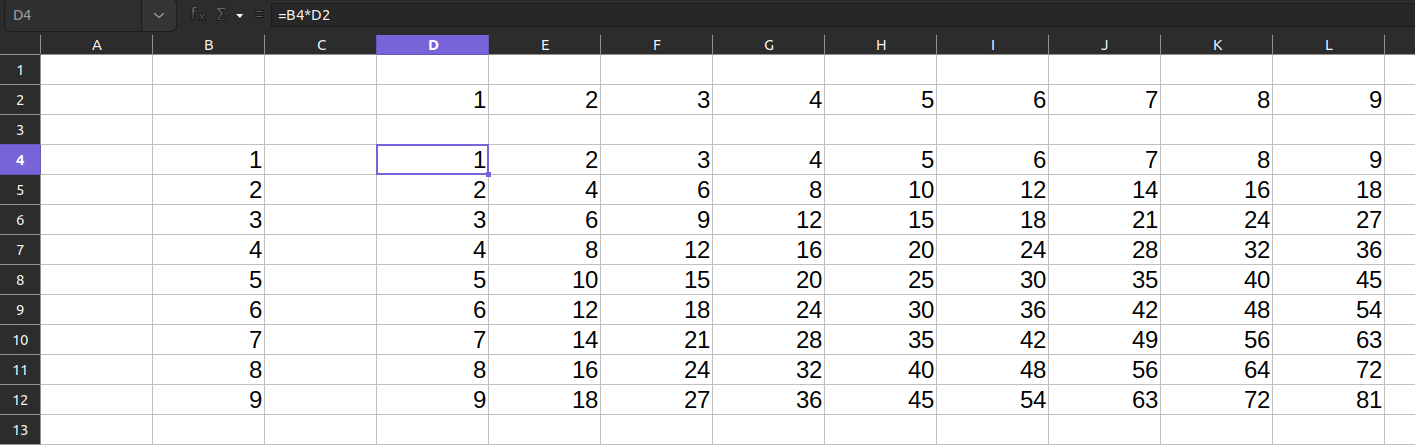
\includegraphics[scale=0.3]{demoValues.png}
  \caption{Multiplication table}
  \label{example2:tableValues}
\end{figure}

\begin{figure}[h]
  \centering
  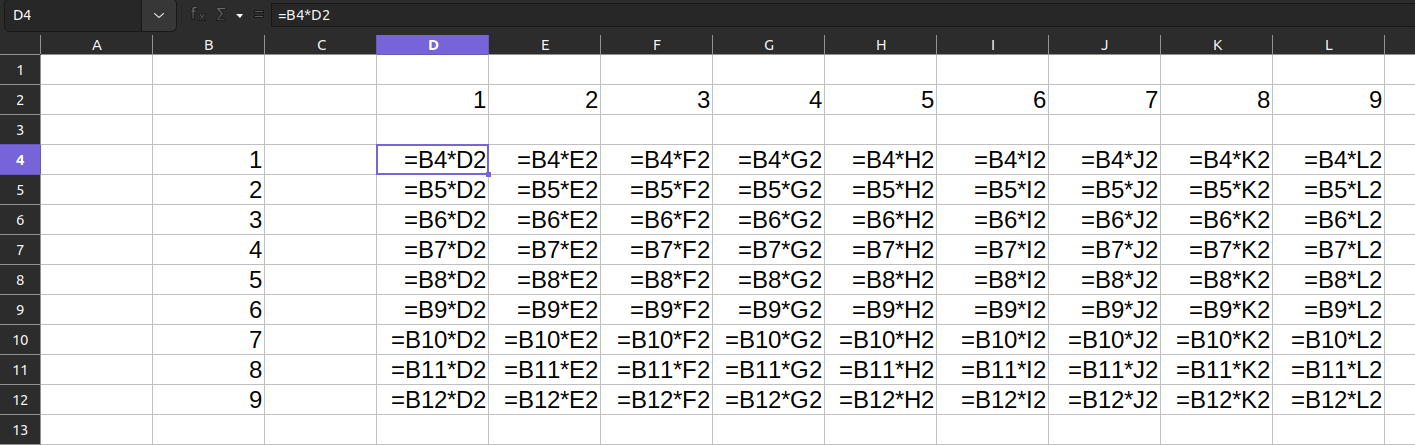
\includegraphics[scale=0.3]{demoFormulas.png}
  \caption{Multiplication table with formulas}
  \label{example2:tableFormulas}
\end{figure}

\subsection{Language Extensions}

First, I enabled the extension that simplified the work with string literals.

\begin{listing}[!h]
  \begin{minted}{haskell}
  {-# LANGUAGE OverloadedStrings #-}
\end{minted}
  \caption{Language extensions}
  \label{example2:languageExtensions}
\end{listing}

\subsection{Imports}

Then, I imported the necessary modules.
Here, I included \hs{Control.Monad} as the task required performing repetitive monadic actions.
The module \hs{Data.Text} was used for constructing sheet names.
The \hs{Lens.Micro} module provided optics for working with cell references.

\begin{listing}[!h]
  \begin{minted}{haskell}
  import Clerk
  import Control.Monad (forM, forM_, void)
  import qualified Data.Text as T
  import Lens.Micro ((&), (+~), (^.))
\end{minted}
  \caption{Imports}
  \label{example2:imports}
\end{listing}

\subsection{Tables}

\newcommand{\vh}{Vertical Header}
\newcommand{\hh}{Horizontal Header}

In my case, a table was a logically grouped set of cell references.
Each table should contain at least a single cell.
The tables that I constructed were the following:

\begin{itemize}
  \item A column with row numbers ("\vh");
  \item A row with column numbers ("\hh");
  \item Tables with results of multiplication of the numbers from these headers ("Inner Table").
\end{itemize}

\subsubsection{\vh}
\label{example2:verticalHeaderSection}

I planned to build a \vh as in \cref{example2:verticalHeader}.

\begin{figure}[h]
  \centering
  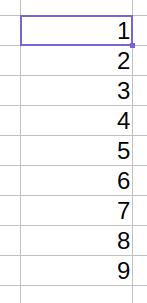
\includegraphics[scale=0.3]{vertical.png}
  \caption{\vh}
  \label{example2:verticalHeader}
\end{figure}

To achieve this goal, I had used the \clerk monadic interface to constructing rows and setting their positions within a sheet.

One of the monads provided by \clerk was the \hs{RowI} monad. Its name meant that inside that monad, I had to use a projection function from an \hs{input} type to \hs{CellData} type. The \hs{CellData} type was the type of spreadsheet values.

The effect of the \hs{RowI} monad was writing a template of a horizontal block of cells. The values obtained from \hs{input} via the projection function were placed onto a sheet according to that template.

I used the monadic function \hs{columnF} for constructing a \hs{RowI}. This function:
\begin{itemize}
  \item added a projected value into the template;
  \item added the formatting to the template;
  \item shifted a pointer to the next free cell in a template.
\end{itemize}

A vertical header contained just a single cell in each its row (\cref{example2:verticalHeader}). Such a header could be represented as several rows with verticall offset equal to \hs{1}. So, the rows were below each other.

I used a \hs{RowI} with one integer as an \hs{input} for a single row cell. This input was the index of the row within the \vh. I set the cell formatting to \hs{blank} since I did not need styling. I placed the rows for each input value onto a \hs{Sheet} and collected the references.

The placement of rows depended on input reference \hs{ref}. I could shift the rows within a sheet by varying this reference. Additionally, I decided to shift all rows vertically by \hs{2} from the input reference.

That said, the function \hs{mkVertical} (\cref{example2:verticalHeaderCode}) for each number from a given range of numbers (size of the multiplication table) and for each index of such a number runs a monadic function in the \hs{Sheet} monad via \hs{forM}. This function \hs{placeIn} at \hs{ref} shifted by \hs{index + 2} vertically places a number according to a \hs{RowI} produced by \hs{columnF}. \hs{columnF} makes a blank cell and uses a constant function as a projection function from the \hs{input} type of \hs{RowI} which is \hs{Int} in this case.

\begin{listing}[!h]
  \begin{minted}{haskell}
mkVertical :: Ref () -> [Int] -> Sheet [Ref Int]
mkVertical ref numbers =
  forM (zip [0 ..] numbers) $ \(idx, number) ->
    placeIn
    (ref & row +~ idx + 2)
    number
    ((columnF blank (const number)) :: RowI Int (Ref Int))
\end{minted}
  \caption{\vh}
  \label{example2:verticalHeaderCode}
\end{listing}

\subsubsection{\hh}
\label{example2:horizontalHeaderSection}

Next, I added a \hh (\Cref{example2:horizontalHeader}).

\begin{figure}[h]
  \centering
  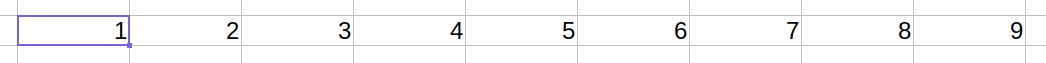
\includegraphics[scale=0.3]{horizontal.png}
  \caption{\hh}
  \label{example2:horizontalHeader}
\end{figure}

I made a row of numbers and collected the references to all its cells (\cref{example2:horizontalHeaderCode}). As the type of inputs was not important, I used the \hs{Row} type. This type assumed that the \hs{input} type was unit, or \hs{()}. In the \hs{Sheet} monad, I placed this row starting at a cell that was shifted horizontally by \hs{2} from the input reference. In this case, I used \hs{forM} to run the monadic function \hs{columnF} several times in the \hs{Row} monad.

\begin{listing}[!h]
  \begin{minted}{haskell}
mkHorizontal :: Ref () -> [Int] -> Sheet [Ref Int]
mkHorizontal ref numbers =
  place
  (ref & col +~ 2)
  ((forM numbers $ \n -> columnF blank (const n)) :: Row [Ref Int])
\end{minted}
  \caption{\hh}
  \label{example2:horizontalHeaderCode}
\end{listing}

\subsubsection{Inner Table}

The next step was to construct a table (\cref{example2:table}).

\begin{figure}[h]
  \centering
  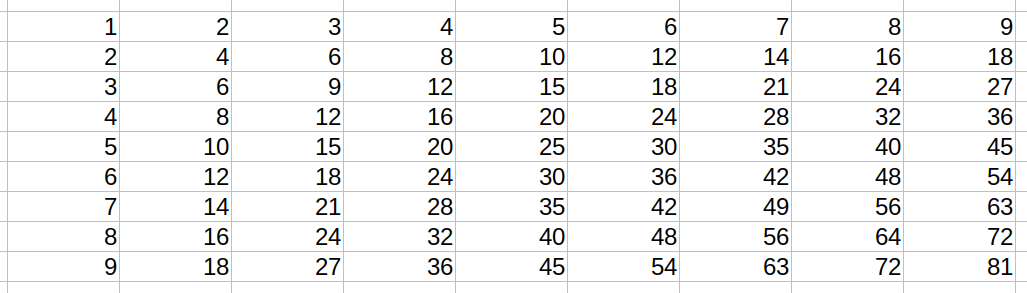
\includegraphics[scale=0.25]{table.png}
  \caption{Inner Table}
  \label{example2:table}
\end{figure}

The function \hs{mkTable} (\cref{example2:tableCode}) took a list of references to cells from the \vh and the \hh. For each such pair of references, it monadically made a coordinate via \hs{mkCoords}. This way, the \hs{mkCoords} function could access the current state of a \hs{Sheet}, e.g., its name and the workbook file path.

I decided to use single-cell rows for each Inner Table cell. This way, I could better align the positions of Inner Table cells with those of cells from headers. Moreover, I used the \hs{Row ()} type since I did not plan to use the references to table cells in other places.

The \hs{columnF} function used a projection to the formula \hs{r .* c}.
In other words, the reference to a cell from the \vh multiplied by the reference to a cell from the \hh.

\begin{listing}[!h]
  \begin{minted}{haskell}
mkTable :: [(Ref Int, Ref Int)] -> Sheet ()
mkTable cs =
  forM_ cs $ \(r, c) -> do
    coords <- mkCoords (c ^. col) (r ^. row)
    place coords ((columnF_ blank (const (r .* c))) :: Row ())  
\end{minted}
  \caption{Inner Table}
  \label{example2:tableCode}
\end{listing}

\subsection{Sheet}

Finally, I produced a complete \hs{Sheet ()}.
Here, I set the initial reference at \hs{B2}.
Then, I produced a list of numbers and constructed the headers.
Lastly, I used a list comprehension to generate all pairs of references to header cells and run \hs{mkTable} on this list of pairs.

\begin{listing}[!h]
  \begin{minted}{haskell}
sheet :: Sheet ()
sheet = do
  start <- mkRef' @"B2"
  let numbers = [1 .. 9]
  cs <- mkHorizontal start numbers
  rs <- mkVertical start numbers
  mkTable [(r, c) | r <- rs, c <- cs]
\end{minted}
  \caption{Inner Table}
  \label{example2:sheetCode}
\end{listing}

\subsection{Result}

To observe the resulting sheet, I run the \hs{main} function from \cref{example2:mainCode}.

\begin{listing}[!h]
  \begin{minted}{haskell}
main :: IO ()
main = writeXlsx "example2.xlsx" [(T.pack "List 1", void sheet)]
\end{minted}
  \caption{Writing result}
  \label{example2:mainCode}
\end{listing}

The resulting table looked as in \cref{example2:table}.
\section{Example 3. Volume and Pressure table}

Sometimes, a user may want to style her generated spreadsheet.
This example shows how to model a problem domain and style the generated spreadsheet.

\subsection{The goal}

The goal was to generate a spreadsheet that calculated the pressure data given volume data and several constants.

The final spreadsheet had the form as in \Cref{fig:volumePressure}.

\begin{figure}[h]
  \centering
  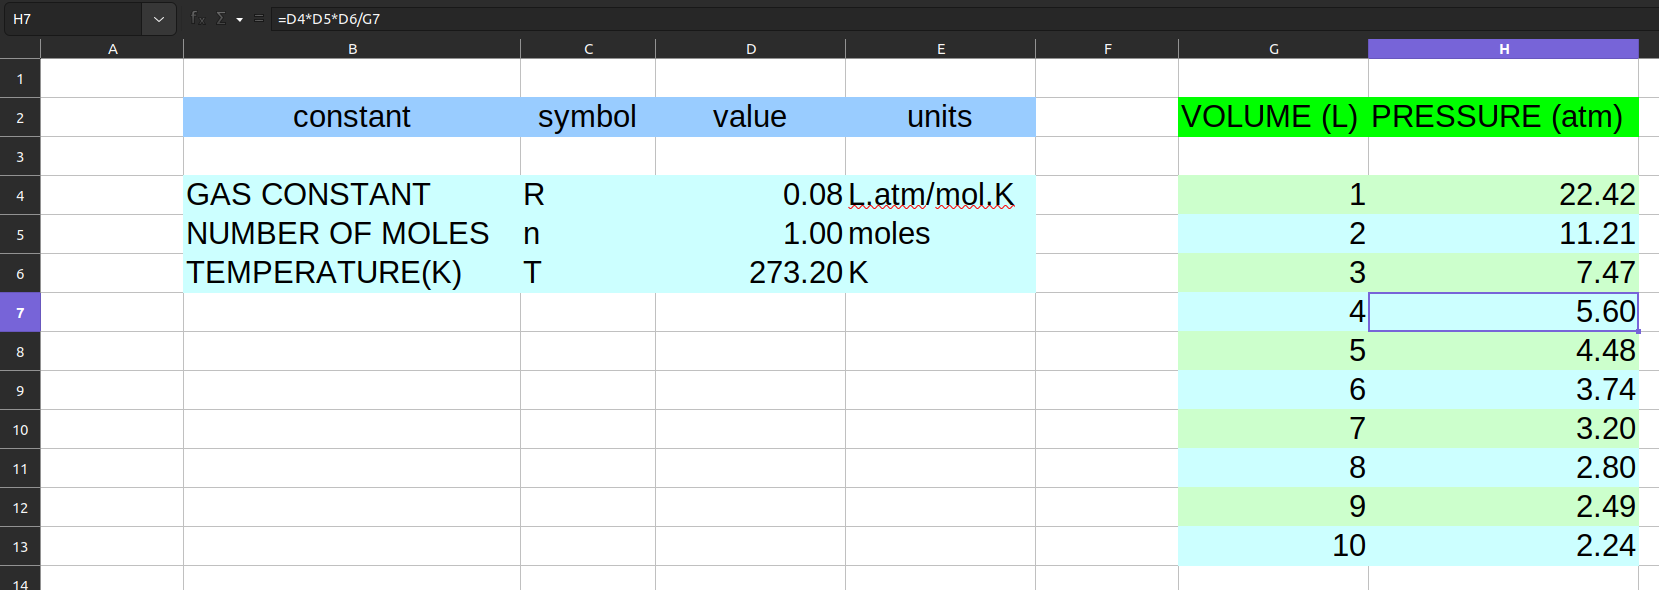
\includegraphics[scale=0.3]{Chapter4/volumePressure.png}
  \caption{Volume and pressure table}
  \label{fig:volumePressure}
\end{figure}

With formulas enabled, I obtained a spreadsheet as in \Cref{fig:volumePressureFormulas}.

\begin{figure}[h]
  \centering
  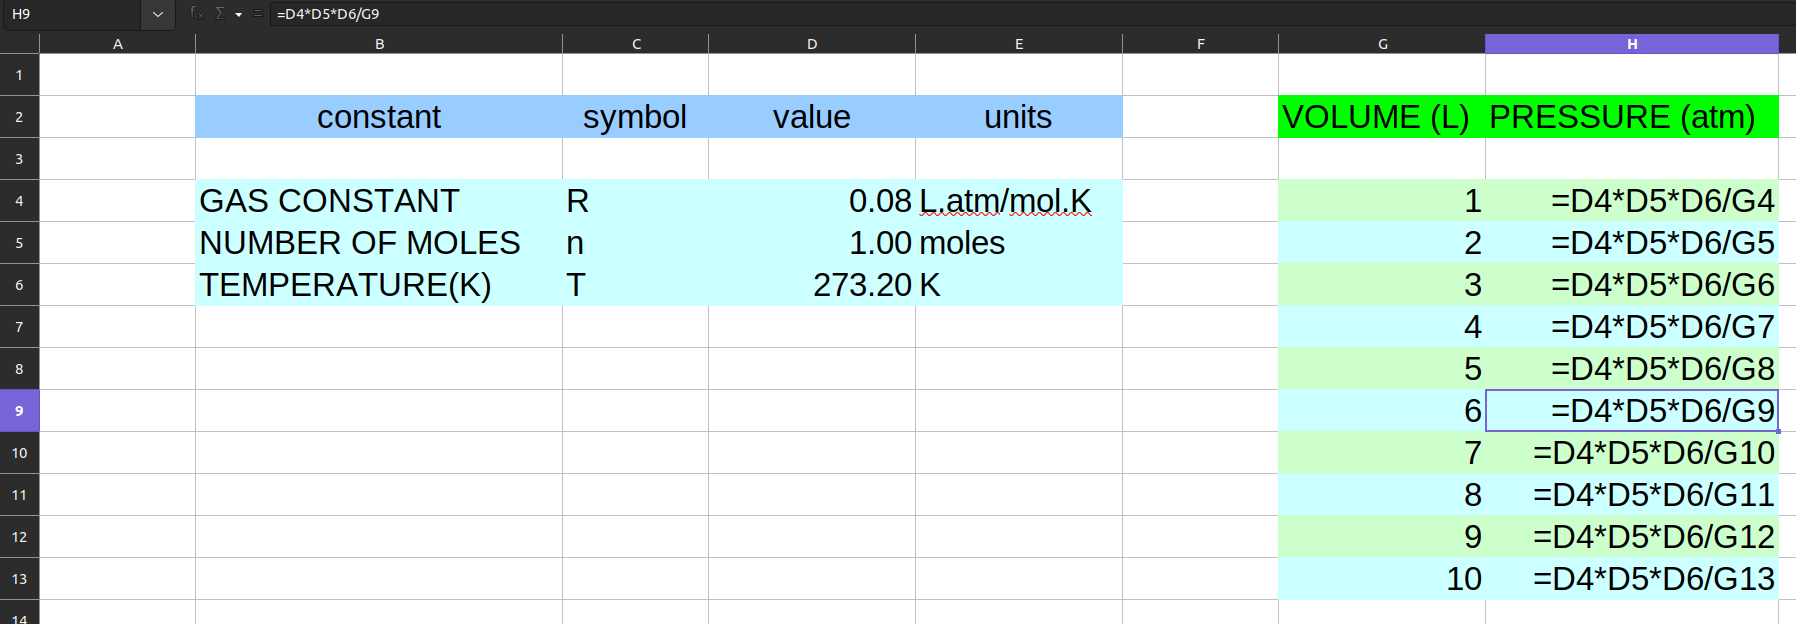
\includegraphics[scale=0.3]{Chapter4/volumePressureFormulas.png}
  \caption{Volume and pressure table with formulas enabled}
  \label{fig:volumePressureFormulas}
\end{figure}

\subsection{Language Extensions}

First, I enabled several language extensions.
\begin{itemize}
  \item \hs{DataKinds} allowed to promote values to type level.
  \item \hs{DuplicateRecordFields} allowed to use the same field names in multiple record data types.
  \item \hs{ImportQualifiedPost} allowed to use module imports of a specific form.
  \item \hs{OverloadedRecordDot} allowed to use the \hs{.} operator for accessing the record fields.
  \item \hs{RecordWildCards} allowed to omit the field names in records in certain cases.
\end{itemize}

\begin{listing}[!h]
  \begin{minted}{haskell}
{-# LANGUAGE DataKinds #-}
{-# LANGUAGE DuplicateRecordFields #-}
{-# LANGUAGE ImportQualifiedPost #-}
{-# LANGUAGE OverloadedRecordDot #-}
{-# LANGUAGE RecordWildCards #-}
{-# LANGUAGE TypeApplications #-}
\end{minted}
\caption{Language extensions}
\label{example3:extensions}
\end{listing}

\subsection{Imports}

Next, I imported the necessary Modules.

\begin{listing}[!h]
  \begin{minted}{haskell}
import Clerk
import Codec.Xlsx qualified as X
import Codec.Xlsx.Formatted qualified as X
import Lens.Micro ((%~), (&), (+~), (?~))
\end{minted}
\caption{Imports}
\label{example3:imports}
\end{listing}

\subsection{Tables}

The tables that I was going to construct were:

- A table per a constant's value (three of them)
- A volume and pressure table
- A constants' header
- A volume and pressure header

\subsubsection{Constants values}

\begin{figure}[h]
  \centering
  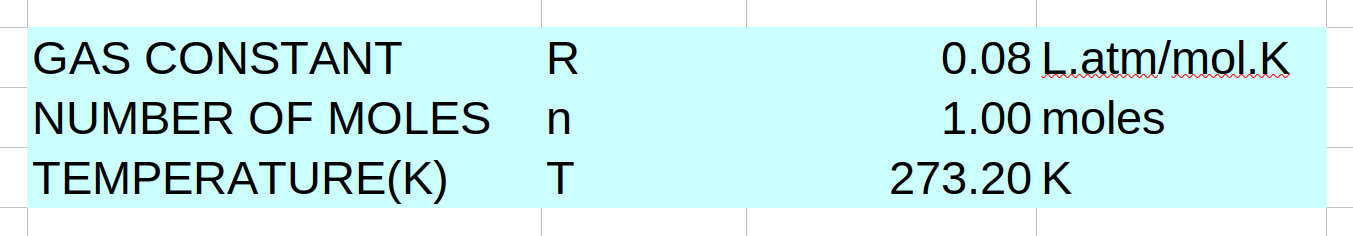
\includegraphics[scale=0.3]{Chapter4/constants.png}
  \caption{Constants values table}
  \label{fig:constants}
\end{figure}

In my case, each constant had the same type of the numeric value - `Double`.
That is why, I constructed a table with a single row per a constant and later placed the constants' tables under each other. I stored constant data in a record.

\begin{listing}[!h]
  \begin{minted}{haskell}
data ConstantData a = ConstantData
  { constantName :: String
  , constantSymbol :: String
  , constantValue :: a
  , constantUnits :: String
  }
\end{minted}
\caption{Constant data}
\label{example3:constantData}
\end{listing}

Next, I grouped the constants into a record. The parameter \texttt{f} may be an arbitrary type of kind \texttt{* -> *}.

\begin{listing}[!h]
  \begin{minted}{haskell}
data Constants f = Constants
  { gasConstant :: f Double
  , numberOfMoles :: f Double
  , temperature :: f Double
  }

type ConstantsInput = Constants ConstantData
\end{minted}
\caption{Constants}
\label{example3:constants}
\end{listing}

Following that, I recorded the constants data.

\begin{listing}[!h]
  \begin{minted}{haskell}
constants :: ConstantsInput
constants =
  Constants
    { gasConstant =
        ConstantData "GAS CONSTANT" "R" 0.08206 "L.atm/mol.K"
    , numberOfMoles =
        ConstantData "NUMBER OF MOLES" "n" 1 "moles"
    , temperature =
        ConstantData "TEMPERATURE(K)" "T" 273.2 "K"
    }
\end{minted}
\caption{Constant values}
\label{example3:constantValues}
\end{listing}

Now, I made a \texttt{RowI} for a constant input.
I used a \texttt{RowI} because this row requires the input type.
I would later use this row for each constant separately.

I got a pair of outputs:

- Top left cell of a constant table. That is, the cell with that constant name.
- The value of the constant.

Later, I would use these outputs to relate the positions of tables on a sheet.

Here, I used \texttt{lightBlue} from the \Cref{sec:styles}.

\begin{listing}[!h]
  \begin{minted}{haskell}
constant :: ToCellData a => RowI (ConstantData a) (Ref (), Ref a)
constant = do
  refTopLeft <- columnF lightBlue constantName
  columnF_ lightBlue constantSymbol
  refValue <- columnF (lightBlue .& with2decimalDigits) constantValue
  columnF_ lightBlue constantUnits
  return (refTopLeft, refValue)
\end{minted}
\caption{Language extensions}
\label{example3:constantCode}
\end{listing}

\subsubsection{Volume and pressure values}

\begin{figure}[h]
  \centering
  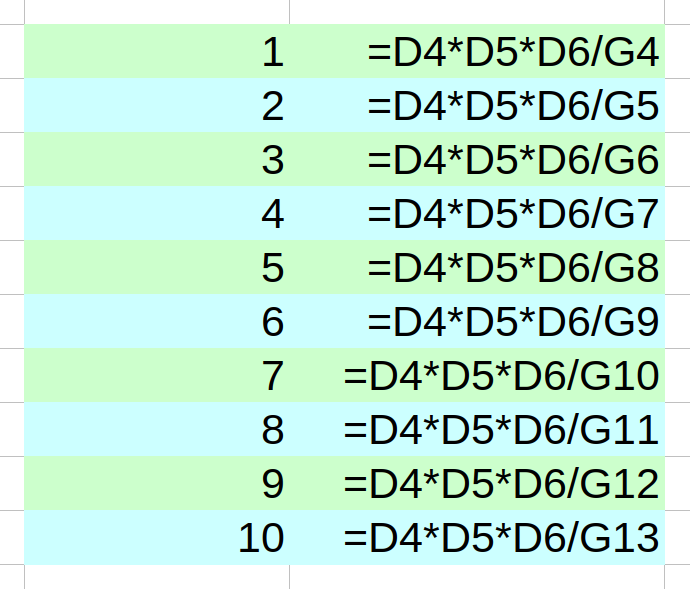
\includegraphics[scale=0.3]{Chapter4/valuesFormulas.png}
  \caption{Volume and pressure table with formulas enabled}
  \label{fig:valuesFormulas}
\end{figure}

I used the data and combined it with the constants to fill table \Cref{fig:valuesFormulas}

\begin{listing}[!h]
  \begin{minted}{haskell}
newtype Volume = Volume {volume :: Double}

volumeData :: [Volume]
volumeData = Volume <$> [1 .. 10]
\end{minted}
\caption{Language extensions}
\label{example3:volumeData}
\end{listing}

I made a helper type to pass the constants references in a structured way.

\begin{listing}[!h]
  \begin{minted}{haskell}
type ConstantsRefs = Constants Ref
\end{minted}
\caption{Constant references}
\label{example3:constantRefs}
\end{listing}

Next, I defined a function to produce a row for volume and pressure.

\begin{listing}[!h]
  \begin{minted}{haskell}
values :: ConstantsRefs -> RowI Volume ()
values Constants{..} = do
  refVolume <- columnF alternatingColors volume
  let pressure' = gasConstant .* numberOfMoles .* temperature ./ refVolume
  columnF_ (alternatingColors .& with2decimalDigits) (const pressure')
\end{minted}
\caption{Values}
\label{example3:valuesCode}
\end{listing}

\subsubsection{Constants' header}

\begin{figure}[h]
  \centering
  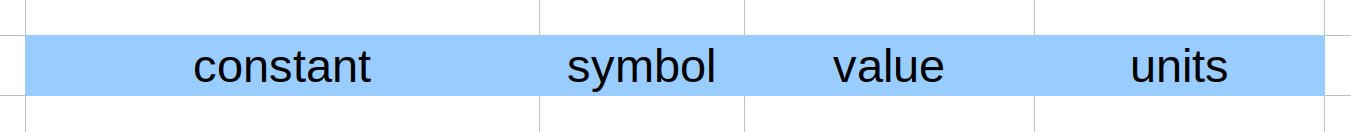
\includegraphics[scale=0.3]{Chapter4/constantsHeader.png}
  \caption{Constants header}
  \label{fig:constantsHeader}
\end{figure}

I did not use records here. Instead, I put the names of the columns straight into the `Row`. The outputs were the coordinates of the top left cell and the top right cell of this table.

\begin{listing}[!h]
  \begin{minted}{haskell}
constantsHeader :: Row (Ref (), Ref ())
constantsHeader = do
  let style :: FormatCell
      style = blue .& alignedCenter
  refTopLeft <- columnWF 20 style (const "constant")
  columnWF_ 8 style (const "symbol")
  columnF_ style (const "value")
  refTopRight <- columnWF 13 style (const "units")
  return (refTopLeft, refTopRight)
\end{minted}
\caption{Language extensions}
\label{example3:extensions}
\end{listing}

\subsubsection{Volume \& Pressure header}

\begin{figure}[h]
  \centering
  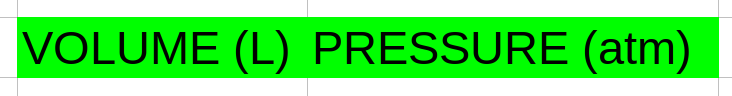
\includegraphics[scale=0.3]{Chapter4/valuesHeader.png}
  \caption{Header for the volume and pressure table}
  \label{fig:valuesHeader}
\end{figure}

For this header, I also put the names of columns straight into a row.

\begin{listing}[!h]
  \begin{minted}{haskell}
valuesHeader :: Row (Ref ())
valuesHeader = do
  refTopLeft <- columnWF 12 green (const "VOLUME (L)")
  columnWF_ 16 green (const "PRESSURE (atm)")
  return refTopLeft
\end{minted}
\caption{Language extensions}
\label{example3:extensions}
\end{listing}

\subsection{Sheet builder}

Finally, I combined all rows.

\begin{listing}[!h]
  \begin{minted}{haskell}
sheet :: Sheet ()
sheet = do
  start <- mkCoords 2 2
  (constantsHeaderTL, constantsHeaderTopRight) <- place start constantsHeader
  (gasTopLeft, gas) <- placeIn (constantsHeaderTL & row +~ 2) constants.gasConstant constant
  (nMolesTopLeft, nMoles) <- placeIn (gasTopLeft & row +~ 1) constants.numberOfMoles constant
  temperature <- snd <$> placeIn (nMolesTopLeft & row +~ 1) constants.temperature constant
  valuesHeaderTopLeft <- place (constantsHeaderTopRight & col +~ 2) valuesHeader
  placeIns (valuesHeaderTopLeft & row +~ 2) volumeData (values $ Constants gas nMoles temperature)
\end{minted}
\caption{Language extensions}
\label{example3:extensions}
\end{listing}

\subsection{Styles}
\label{sec:styles}

Below, I list the expressions used for sheet styling.

\begin{listing}[!h]
  \begin{minted}{haskell}
blue, lightBlue, green, lightGreen :: FormatCell
blue = mkColor (hex @"#FF99CCFF")
lightBlue = mkColor (hex @"#90CCFFFF")
green = mkColor (hex @"#FF00FF00")
lightGreen = mkColor (hex @"#90CCFFCC")

alternatingColors :: FormatCell
alternatingColors index = (if even index then lightGreen else lightBlue) index
\end{minted}
\caption{Language extensions}
\label{example3:extensions}
\end{listing}

Additionally, I composed an \texttt{FCTransform} for the number format.
Such a transform was used to accumulate cell formatting.

\begin{listing}[!h]
  \begin{minted}{haskell}
with2decimalDigits :: FCTransform
with2decimalDigits fcTransform =
  fcTransform & X.formattedFormat %~ X.formatNumberFormat ?~ X.StdNumberFormat X.Nf2Decimal
\end{minted}
\caption{Language extensions}
\label{example3:extensions}
\end{listing}

Finally, I made a transform for centering the cell contents.

\begin{listing}[!h]
  \begin{minted}{haskell}
alignedCenter :: FCTransform
alignedCenter = horizontalAlignment X.CellHorizontalAlignmentCenter
\end{minted}
\caption{Language extensions}
\label{example3:extensions}
\end{listing}

% \include{chapters/chapter4-3.tex}
% \include{chapters/chapter4-cont}
% \include{chapters/chap}
% \chapter{Evaluation and Discussion}
\label{chap:eval}

This chapter analyzes the research results.

\Cref{eval:findings} presents the main findings that are connected with the research purpose.
\Cref{eval:finding-results} interprets how the research results support these findings.
\Cref{eval:previous-research} contrasts my findings with the results of the past researches.
\Cref{eval:discrepancies} explains the discrepancies between my results and findings.
\Cref{eval:limitations} describes the limitations of my research.
\Cref{eval:unexpected} lists the unexpected findings.
\Cref{eval:outer-applications} suggests the possible applications of my research findings.

\section{Key findings}
\label{eval:findings}


The main finding is that it is possible to build a Haskell eDSL as a library that allows for declarative spreadsheet construction.
A user specifies the connections between the spreadsheet elements, and the library functions produce the elements layout automatically.
Despite being simple, the language requires the knowledge of Haskell at least at the beginner level.
That is why, the target audience of the language is Haskell programmers.
They are expected to generate the spreadsheets and pass these spreadsheets to non-programmers.

Another finding is that such an eDSL provides the means to construct statically typed formulas.
This feature allows for typechecking the formula expressions at compile time.
Such checks prevent runtime errors, such as invalid formula arguments, in spreadsheet applications.

The third finding is that it is possible to use the existing Haskell features in the programs written in the new eDSL.
First, formulas can be curried, composed, and applied to ranges of values and cell references.
Second, algebraic data types can be used to model the value domains.
Third, the \texttt{do-notation} works because the eDSL has a monadic interface.

\section{Results and findings}
\label{eval:finding-results}

First, the result of my research is the \texttt{clerk} Haskell package.
It is publicly available on GitHub \cite{danko_clerk_2023} and Hackage \cite{hackage_clerk_2023}.
Haskell programmers may discover the package there, read through the examples from the package description and use \texttt{clerk} in their programs.
The examples are based on simple problems and demonstrate most features of the eDSL.

Second, the type checking of formulas works at compile time.
A user first specifies the formula signature - a name and the types of arguments.
Later, the user can apply a formula to arguments.

Third, the examples from the package description demonstrate how to apply certain Haskell features to write type-safe monadic code using \texttt{clerk}.

\section{Previous research}
\label{eval:previous-research}

Currently, the major spreadsheet applications provide limited tools for declarative type-safe construction of spreadsheets.

\subsection{User-defined data types}
\label{subsec:user-defined-data-types}
Firstly, Microsoft Excel provides creation of user-defined data types \cite{excel_custom_types}.
A user may group the columns of values into records that represent user-defined types.
Additionally, they may use a user-defined data type as a type of a field of another user-defined data type.

In contrast, \texttt{clerk} allows to type-safely group values into Haskell records.
This approach allows for building type-safe composite records before importing them into a spreadsheet application.

\subsection{User-defined functions}

Microsoft Excel introduced the \texttt{LAMBDA} function \cite{excel_lambda} that allows for user-defined functions.
Google Sheets also provides the \texttt{LAMBDA} function \cite{sheets_lambda} that should immediately be applied to a value.
Thus, in this section, I focus on the \texttt{LAMBDA} function from Microsoft Excel.

First, the \texttt{LAMBDA} function can be recorded and shared between spreadsheets.
Second, this function allows for recursion and usage of other functions, including user-defined ones.
Third, user-defined functions are dynamically-typed.
The argument types can be specified as comments to a recorded user-defined function.

In comparison to \texttt{LAMBDA}, \texttt{clerk} allows a user to declare functions in Haskell.
First, these functions can be imported into other Haskell modules or programs.
Second, these functions may represent compositions of functions from the target spreadsheet system, including user-defined ones.
Third, these functions are statically typed. Their arguments may be documented using Haddock.

\subsection{Declarative layout}

Currently, Microsoft Excel has support for automatic layout of data upon importing it \cite{excel_custom_types}.
However, layout customization still should be done manually.

There are libraries for several languages that derive the layout from user specification of spreadsheet elements and the connections between them.
The \texttt{poi} library for Python can write spreadsheets based on user data \cite{wang_poi_nodate}.
To my knowledge, the library does not allow to specify the connections between new eleemnts and previously built elements.



\section{Discrepancies}
\label{eval:discrepancies}

\section{Limitations}
\label{eval:limitations}

\section{Unexpected findings}
\label{eval:unexpected}

\section{Outer applications}
\label{eval:outer-applications}

The \texttt{clerk} library allows to produce correct by construction spreadsheets.
I suppose that this property can make the library useful in real world systems.

First, this library can be used as a part of data pipelines.
The program using the \texttt{clerk} library can generate data-transforming spreadsheets.
There will be regions for input data, output data, and formulas.
The formulas will act onto input data to produce output data.
Other programs may write to or read the outputs from such data-transforming spreadsheets.

Second, such a library may be useful in areas that require correct computations.
As far as I know from Haskell community chats, some financial and biotechnological organizations rely on Haskell.
Moreover, some people use Excel for recording the results of scientific experiments.

Third, it is possible to use \texttt{clerk} for generating reports.
The library provides basic styling capabilities.
When the library is used with a Haskell repl, the resulting spreadsheets can be generated rapidly.
Thus, the spreadsheet editor may quickly observe the changes.

Fourth, the library may be used by pixel art fans.
It is quite trivial to fill the table cells with colors of pixels of an image.

Fifth, the library can be used for teaching type-level programming in Haskell.
More specifically, the library includes modules that provide type-level parsing capabilities.
These modules enable compile-time cell address and color values checks.

% \begin{longtable}{c|c}
% \caption[This is the title I want to appear in the List of Tables]{Simulation Parameters} \label{table:fifsimulation_params} \\
% \hline
% A & B  \\
% \hline
% \endfirsthead
% \multicolumn{2}{@{}l}{} \\
% \hline
% A & B \\
% \hline
% \endhead
% \hline
%  \textbf{Parameter} & \textbf{Value}\\
%  \hline
%  Number of vehicles & $|\mathcal{V}|$\\
%  \hline
%  Number of RSUs & $|\mathcal{U}|$\\
%  \hline
%  RSU coverage radius & 150 m\\
%  \hline
%  V2V communication radius & 30 m\\
%  \hline
%  Smart vehicle antenna height & 1.5 m\\
%  \hline
%  RSU antenna height & 25 m\\
%  \hline
%  Smart vehicle maximum speed & $v_{max}$ m/s\\
%  \hline
%  Smart vehicle minimum speed & $v_{min}$ m/s\\
%  \hline
%  Common smart vehicle cache capacities & $[50, 100, 150, 200, 250]$ mb\\
%  \hline
%  Common RSU cache capacities & $[5000,1000,1500,2000,2500]$ mb\\
%  \hline
%  Common backhaul rates & $[75, 100, 150]$ mb/s\\
%  \hline
% \end{longtable}

% \begin{figure}[hbt]
% \centering
% 
\includegraphics[]{figs/inno.png}
% \caption{One kernel at $x_s$ (\emph{dotted kernel}) or two kernels at
% $x_i$ and $x_j$ (\textit{left and right}) lead to the same summed estimate
% at $x_s$. This shows a figure consisting of different types of
% lines. Elements of the figure described in the caption should be set in
% italics, in parentheses, as shown in this sample caption.}
% \label{fig:fifex}
% \end{figure}

\ldots

%\chapter{Conclusion}
\label{chap:conclusion}
\begin{longtable}{c|c}
\caption[This is the title I want to appear in the List of Tables]{Simulation Parameters} \label{table:sixsimulation_params} \\
\hline
A & B  \\
\hline
\endfirsthead
\multicolumn{2}{@{}l}{} \\
\hline
A & B \\
\hline
\endhead
\hline
 \textbf{Parameter} & \textbf{Value}\\
 \hline
 Number of vehicles & $|\mathcal{V}|$\\
 \hline
 Number of RSUs & $|\mathcal{U}|$\\
 \hline
 RSU coverage radius & 150 m\\
 \hline
 V2V communication radius & 30 m\\
 \hline
 Smart vehicle antenna height & 1.5 m\\
 \hline
 RSU antenna height & 25 m\\
 \hline
 Smart vehicle maximum speed & $v_{max}$ m/s\\
 \hline
 Smart vehicle minimum speed & $v_{min}$ m/s\\
 \hline
 Common smart vehicle cache capacities & $[50, 100, 150, 200, 250]$ mb\\
 \hline
 Common RSU cache capacities & $[5000,1000,1500,2000,2500]$ mb\\
 \hline
 Common backhaul rates & $[75, 100, 150]$ mb/s\\
 \hline
\end{longtable}

\begin{figure}[hbt]
\centering

\includegraphics[]{figs/inno.png}
\caption{One kernel at $x_s$ (\emph{dotted kernel}) or two kernels at
$x_i$ and $x_j$ (\textit{left and right}) lead to the same summed estimate
at $x_s$. This shows a figure consisting of different types of
lines. Elements of the figure described in the caption should be set in
italics, in parentheses, as shown in this sample caption.}
\label{fig:sixex}
\end{figure}

\ldots



%% REFERENCES
\printbibliography[heading=bibintoc,title={Bibliography cited}]
% \appendix
\chapter{Extra Stuff}
\blindtext

\chapter{Even More Extra Stuff}
\blindtext
\end{document}

